% Source PDF page 81 (printed p. 67)
\chapter{凸函数}
\section{基本性质与例子}
\subsection{定义}
若函数 $f:\R^n\to\R$ 的定义域 $\dom f$ 是凸集，并且对所有 $x,y\in\dom f$ 以及 $0\leq\theta\leq1$，都有
\begin{equation}
 f(\theta x+(1-\theta)y)\leq\theta f(x)+(1-\theta)f(y),\tag{3.1}
\end{equation}
则称 $f$ 为凸函数。

从几何上说，这个不等式意味着，连接 $(x,f(x))$ 与 $(y,f(y))$ 的线段，也就是从 $x$ 到 $y$ 的弦，位于 $f$ 的图像上方（图3.1）。如果只要 $x\ne y$ 且 $0<\theta<1$，式(3.1)中的不等号就严格成立，则称 $f$ 为严格凸函数。若 $-f$ 凸，则称 $f$ 凹；若 $-f$ 严格凸，则称 $f$ 严格凹。

对于仿射函数，式(3.1)总取等号，因此所有仿射函数（从而也包括所有线性函数）都既凸又凹。反过来，既凸又凹的函数必为仿射函数。

一个函数是凸函数，当且仅当把它限制在任意与其定义域相交的直线上时，所得函数都凸。换句话说，$f$ 凸，当且仅当对所有 $x\in\dom f$ 和所有 $v$，函数 $g(t)=f(x+tv)$ 在其定义域 $\{t\mid x+tv\in\dom f\}$ 上凸。
\begin{figure}[htbp]\centering
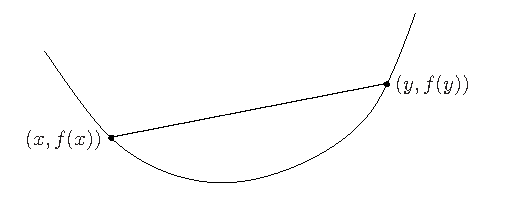
\includegraphics[width=.58\textwidth]{figures/ch03-81.pdf}
\caption*{图3.1 凸函数的图像。连接图像上任意两点的弦（即线段）都位于图像上方。}
\end{figure}
% Source PDF page 82 (printed p. 68)
这一性质很有用，因为它使我们能够通过将函数限制在直线上，检查函数的凸性。

凸函数分析是一个发展完善的领域，本书不作深入讨论。例如，一个简单结论是：凸函数在其定义域的相对内部连续；不连续只能出现在相对边界上。

\subsection{扩展值延拓}
把凸函数在定义域外的值定义为 $\infty$，从而将它延拓到整个 $\R^n$，往往很方便。若 $f$ 凸，定义其扩展值延拓 $\widetilde f:\R^n\to\R\cup\{\infty\}$ 为
\[
 \widetilde f(x)=\begin{cases}f(x),&x\in\dom f,\\ \infty,&x\notin\dom f.\end{cases}
\]
延拓 $\widetilde f$ 在整个 $\R^n$ 上有定义，取值于 $\R\cup\{\infty\}$。原函数的定义域可以从延拓恢复：$\dom f=\{x\mid\widetilde f(x)<\infty\}$。

延拓可以简化记号，因为我们不必显式描述定义域，也不必每次提到 $f(x)$ 时都加上“对所有 $x\in\dom f$”这一限定。例如，基本定义不等式(3.1)用延拓 $\widetilde f$ 可以写为：当 $0<\theta<1$ 时，对任意 $x,y$ 都有
\[
 \widetilde f(\theta x+(1-\theta)y)
 \leq\theta\widetilde f(x)+(1-\theta)\widetilde f(y).
\]
（当 $\theta=0$ 或 $\theta=1$ 时，不等式总成立。）这里当然必须用扩展算术与次序来理解不等式。若 $x,y$ 都属于 $\dom f$，它就与式(3.1)相同；若其中一点在定义域外，则右端为 $\infty$，因此不等式成立。

再看这种记号用法的另一个例子。设 $f_1,f_2$ 是 $\R^n$ 上的两个凸函数。逐点和 $f=f_1+f_2$ 的定义域为 $\dom f=\dom f_1\cap\dom f_2$，且对任意 $x\in\dom f$ 有 $f(x)=f_1(x)+f_2(x)$。用扩展值延拓，我们只需说，对任意 $x$ 都有 $\widetilde f(x)=\widetilde f_1(x)+\widetilde f_2(x)$。在此等式中，$f$ 的定义域自动成为 $\dom f_1\cap\dom f_2$，因为只要 $x\notin\dom f_1$ 或 $x\notin\dom f_2$，就有 $\widetilde f(x)=\infty$。这个例子利用扩展算术自动确定了定义域。

在本书中，只要歧义不会造成问题，就用同一个符号表示凸函数及其延拓。这相当于假定所有凸函数都已隐式延拓，即在定义域外取值 $\infty$。

\begin{origexample}{3.1}
\textbf{凸集的示性函数。}设 $C\subseteq\R^n$ 为凸集，考虑定义域为 $C$、在所有 $x\in C$ 处满足 $I_C(x)=0$ 的凸函数 $I_C$。换句话说，这个函数在 $C$ 上恒为零。它的扩展值延拓为
% Source PDF page 83 (printed p. 69)
\[
 \widetilde I_C(x)=\begin{cases}0,&x\in C,\\ \infty,&x\notin C.\end{cases}
\]
凸函数 $\widetilde I_C$ 称为集合 $C$ 的示性函数。

示性函数 $\widetilde I_C$ 可以带来几种方便的记号处理。例如，在集合 $C$ 上最小化函数 $f$（不妨设它在整个 $\R^n$ 上有定义），等同于在整个 $\R^n$ 上最小化函数 $f+\widetilde I_C$。事实上，按我们的约定，$f+\widetilde I_C$ 就是 $f$ 在 $C$ 上的限制。
\end{origexample}
类似地，可令凹函数在定义域外取值 $-\infty$，得到它的延拓。
\begin{figure}[htbp]\centering
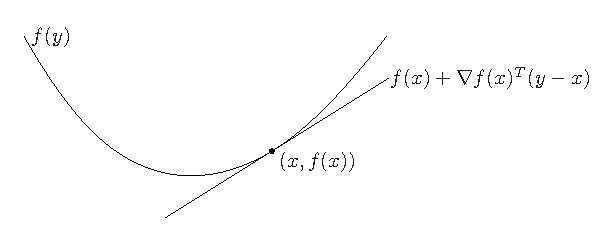
\includegraphics[width=.65\textwidth]{figures/ch03-83.pdf}
\caption*{图3.2 若 $f$ 凸且可微，则对所有 $x,y\in\dom f$ 都有 $f(x)+\nabla f(x)^\T(y-x)\leq f(y)$。}
\end{figure}
\subsection{一阶条件}
假设 $f$ 可微，即它的梯度 $\nabla f$ 在开集 $\dom f$ 中的每一点都存在。那么，$f$ 凸，当且仅当 $\dom f$ 凸，且对所有 $x,y\in\dom f$ 都有
\begin{equation}
 f(y)\geq f(x)+\nabla f(x)^\T(y-x).\tag{3.2}
\end{equation}
图3.2说明了这个不等式。

关于 $y$ 的仿射函数 $f(x)+\nabla f(x)^\T(y-x)$，正是 $f$ 在 $x$ 附近的一阶 Taylor 近似。不等式(3.2)表明：对于凸函数，一阶 Taylor 近似实际上是函数的全局下估计。反过来，如果函数的一阶 Taylor 近似总是全局下估计，则该函数凸。

不等式(3.2)表明，从凸函数的局部信息（即某一点的函数值与导数）能够导出全局信息（即全局下估计）。这也许是凸函数最重要的性质，并解释了凸函数及凸优化问题的一些突出特点。举一个简单例子，由式(3.2)，若 $\nabla f(x)=0$，则对所有 $y\in\dom f$ 都有 $f(y)\geq f(x)$，也就是说，$x$ 是函数 $f$ 的一个全局最小点。
% Source PDF page 84 (printed p. 70)
严格凸性也可以用一阶条件刻画：$f$ 严格凸，当且仅当 $\dom f$ 凸，且对 $x,y\in\dom f$、$x\ne y$ 有
\begin{equation}
 f(y)>f(x)+\nabla f(x)^\T(y-x).\tag{3.3}
\end{equation}
对于凹函数有相应刻画：$f$ 凹，当且仅当 $\dom f$ 凸，并且对所有 $x,y\in\dom f$ 都有
\[f(y)\leq f(x)+\nabla f(x)^\T(y-x).\]

\subsubsection*{凸性一阶条件的证明}
为证明式(3.2)，先考虑 $n=1$ 的情形。我们将证明，可微函数 $f:\R\to\R$ 凸，当且仅当对定义域内所有 $x,y$ 都有
\begin{equation}
 f(y)\geq f(x)+f'(x)(y-x).\tag{3.4}
\end{equation}
先设 $f$ 凸且 $x,y\in\dom f$。由于 $\dom f$ 凸（即为区间），对所有 $0<t\leq1$ 都有 $x+t(y-x)\in\dom f$，再由 $f$ 的凸性得到
\[f(x+t(y-x))\leq(1-t)f(x)+tf(y).\]
两边除以 $t$ 并整理，得到
\[f(y)\geq f(x)+\frac{f(x+t(y-x))-f(x)}{t}.\]
令 $t\to0$，即得式(3.4)。

为证明充分性，假设函数对 $\dom f$（一个区间）中的所有 $x,y$ 都满足式(3.4)。任取 $x\ne y$、$0\leq\theta\leq1$，令 $z=\theta x+(1-\theta)y$。两次应用式(3.4)，得
\[
 f(x)\geq f(z)+f'(z)(x-z),\qquad
 f(y)\geq f(z)+f'(z)(y-z).
\]
第一个不等式乘以 $\theta$，第二个乘以 $1-\theta$，再相加，得到
\[\theta f(x)+(1-\theta)f(y)\geq f(z),\]
这证明了 $f$ 凸。

现在证明一般情形 $f:\R^n\to\R$。设 $x,y\in\R^n$，考虑 $f$ 在经过它们的直线上的限制，即函数 $g(t)=f(ty+(1-t)x)$；其导数为 $g'(t)=\nabla f(ty+(1-t)x)^\T(y-x)$。

先假设 $f$ 凸，则 $g$ 凸。根据上面的论证，有 $g(1)\geq g(0)+g'(0)$，即
\[f(y)\geq f(x)+\nabla f(x)^\T(y-x).\]
再假设这个不等式对任意 $x,y$ 都成立。若 $ty+(1-t)x\in\dom f$ 且 $\widetilde t y+(1-\widetilde t)x\in\dom f$，则
\[
\begin{split}
 f(ty+(1-t)x)\geq{}& f(\widetilde t y+(1-\widetilde t)x)\\
 &+\nabla f(\widetilde t y+(1-\widetilde t)x)^\T(y-x)(t-\widetilde t),
\end{split}
\]
也就是 $g(t)\geq g(\widetilde t)+g'(\widetilde t)(t-\widetilde t)$。前面已经证明，这意味着 $g$ 凸。
% Source PDF page 85 (printed p. 71)
\subsection{二阶条件}
现在假设 $f$ 二次可微，也就是说，它的 Hessian 矩阵或二阶导数 $\nabla^2f$ 在开集 $\dom f$ 的每一点都存在。那么，$f$ 凸，当且仅当 $\dom f$ 凸，且 Hessian 矩阵半正定，即对所有 $x\in\dom f$ 有
\[\nabla^2f(x)\succeq0.\]
对于 $\R$ 上的函数，这简化为 $f''(x)\geq0$（同时 $\dom f$ 凸，即为区间），也就是导数单调不减。几何上，条件 $\nabla^2f(x)\succeq0$ 要求函数图像在 $x$ 处具有正的（向上的）曲率。二阶条件的证明留作习题3.8。

类似地，$f$ 凹，当且仅当 $\dom f$ 凸，且对所有 $x\in\dom f$ 都有 $\nabla^2f(x)\preceq0$。二阶条件也能部分刻画严格凸性：若对所有 $x\in\dom f$ 都有 $\nabla^2f(x)\succ0$，则 $f$ 严格凸。但逆命题不成立；例如，函数 $f:\R\to\R$，$f(x)=x^4$ 严格凸，却在 $x=0$ 处的二阶导数为零。

\begin{origexample}{3.2}
\textbf{二次函数。}考虑定义域为 $\R^n$ 的二次函数 $f:\R^n\to\R$，
\[f(x)=\tfrac12x^\T Px+q^\T x+r,\]
其中 $P\in\mathbb S^n$、$q\in\R^n$、$r\in\R$。由于所有 $x$ 处都有 $\nabla^2f(x)=P$，$f$ 凸当且仅当 $P\succeq0$（凹当且仅当 $P\preceq0$）。

二次函数的严格凸性容易刻画：$f$ 严格凸当且仅当 $P\succ0$（严格凹当且仅当 $P\prec0$）。
\end{origexample}
\paragraph{注3.1}在凸性和凹性的一阶、二阶刻画中，不能省去 $\dom f$ 为凸集这一单独要求。例如，定义域为 $\{x\in\R\mid x\ne0\}$ 的函数 $f(x)=1/x^2$，在所有 $x\in\dom f$ 处都满足 $f''(x)>0$，却不是凸函数。

\subsection{例子}
前面已经提到，所有线性函数和仿射函数都凸（也凹），并描述了凸二次函数与凹二次函数。本节再给出几个凸函数和凹函数的例子。先看 $\R$ 上以 $x$ 为变量的函数。
\begin{itemize}
\item \textbf{指数。}对任意 $a\in\R$，$e^{ax}$ 在 $\R$ 上凸。
\item \textbf{幂。}当 $a\geq1$ 或 $a\leq0$ 时，$x^a$ 在 $\R_{++}$ 上凸；当 $0\leq a\leq1$ 时，它凹。
\item \textbf{绝对值的幂。}当 $p\geq1$ 时，$|x|^p$ 在 $\R$ 上凸。
\item \textbf{对数。}$\log x$ 在 $\R_{++}$ 上凹。
% Source PDF page 86 (printed p. 72)
\item \textbf{负熵。}$x\log x$ 是凸函数，定义域可取 $\R_{++}$，也可取 $\R_+$，后者在 $x=0$ 处定义为零。
\end{itemize}
\begin{figure}[htbp]\centering
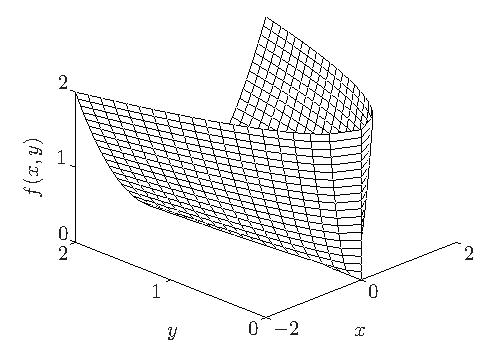
\includegraphics[width=.58\textwidth]{figures/ch03-86.pdf}
\caption*{图3.3 $f(x,y)=x^2/y$ 的图像。}
\end{figure}
这些例子的凸性或凹性，可以通过验证基本不等式(3.1)，或检查二阶导数非负、非正来证明。例如，$f(x)=x\log x$ 有
\[f'(x)=\log x+1,\qquad f''(x)=1/x,\]
所以当 $x>0$ 时 $f''(x)>0$。这说明负熵函数严格凸。

现在给出 $\R^n$ 上几个值得关注的函数例子。
\begin{itemize}
\item \textbf{范数。}$\R^n$ 上的每一个范数都凸。
\item \textbf{最大值函数。}$f(x)=\max\{x_1,\ldots,x_n\}$ 在 $\R^n$ 上凸。
\item \textbf{二次除以线性函数。}$f(x,y)=x^2/y$，定义域为
\[\dom f=\R\times\R_{++}=\{(x,y)\in\R^2\mid y>0\},\]
是凸函数（图3.3）。
\item \textbf{指数和的对数。}$f(x)=\log(e^{x_1}+\cdots+e^{x_n})$ 在 $\R^n$ 上凸。它可以看作最大值函数的可微近似（事实上是解析近似），因为对所有 $x$ 都有
\[
\max\{x_1,\ldots,x_n\}\leq f(x)
 \leq\max\{x_1,\ldots,x_n\}+\log n.
\]
（当 $x$ 的各分量相等时，第二个不等式取等号。）图3.4给出 $n=2$ 时的 $f$。
% Source PDF page 87 (printed p. 73)
\item \textbf{几何平均。}几何平均 $f(x)=(\prod_{i=1}^n x_i)^{1/n}$ 在 $\dom f=\R_{++}^n$ 上凹。
\item \textbf{行列式的对数。}函数 $f(X)=\log\det X$ 在 $\dom f=\mathbb S_{++}^n$ 上凹。
\end{itemize}
\begin{figure}[htbp]\centering
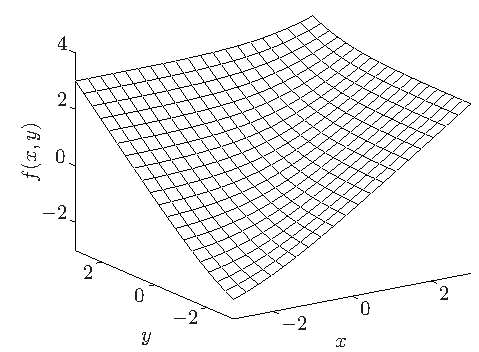
\includegraphics[width=.58\textwidth]{figures/ch03-87.pdf}
\caption*{图3.4 $f(x,y)=\log(e^x+e^y)$ 的图像。}
\end{figure}
这些例子的凸性（或凹性）可以用多种方法验证，例如直接验证不等式(3.1)，检查 Hessian 半正定，或把函数限制在任意一条直线上，再验证所得一元函数的凸性。

\paragraph{范数。}若 $f:\R^n\to\R$ 是范数，且 $0\leq\theta\leq1$，则
\[
 f(\theta x+(1-\theta)y)\leq f(\theta x)+f((1-\theta)y)
 =\theta f(x)+(1-\theta)f(y).
\]
不等式来自三角不等式，等式来自范数的齐次性。

\paragraph{最大值函数。}对 $0\leq\theta\leq1$，函数 $f(x)=\max_i x_i$ 满足
\[
\begin{aligned}
 f(\theta x+(1-\theta)y)&=\max_i(\theta x_i+(1-\theta)y_i)\\
 &\leq\theta\max_i x_i+(1-\theta)\max_i y_i\\
 &=\theta f(x)+(1-\theta)f(y).
\end{aligned}
\]
\paragraph{二次除以线性函数。}为证明 $f(x,y)=x^2/y$ 凸，注意到当 $y>0$ 时，
\[
 \nabla^2f(x,y)=\frac2{y^3}
 \begin{bmatrix}y^2&-xy\\-xy&x^2\end{bmatrix}
 =\frac2{y^3}\begin{bmatrix}y\\-x\end{bmatrix}
 \begin{bmatrix}y\\-x\end{bmatrix}^{\T}\succeq0.
\]
% Source PDF page 88 (printed p. 74)
\paragraph{指数和的对数。}指数和对数函数的 Hessian 为
\[
 \nabla^2 f(x)=\frac1{(\one^\T z)^2}
 \bigl((\one^\T z)\diag(z)-zz^\T\bigr),
\]
其中 $z=(e^{x_1},\ldots,e^{x_n})$。要验证 $\nabla^2f(x)\succeq0$，必须证明对所有 $v$ 有 $v^\T\nabla^2f(x)v\geq0$，即
\[
 v^\T\nabla^2f(x)v=\frac1{(\one^\T z)^2}
 \left(\left(\sum_{i=1}^n z_i\right)\left(\sum_{i=1}^n v_i^2z_i\right)
 -\left(\sum_{i=1}^n v_iz_i\right)^2\right)\geq0.
\]
对分量为 $a_i=v_i\sqrt{z_i}$、$b_i=\sqrt{z_i}$ 的向量应用 Cauchy--Schwarz 不等式 $(a^\T a)(b^\T b)\geq(a^\T b)^2$，便得到所需结论。

\paragraph{几何平均。}类似地，可以证明几何平均 $f(x)=(\prod_{i=1}^n x_i)^{1/n}$ 在 $\dom f=\R_{++}^n$ 上凹。它的 Hessian $\nabla^2f(x)$ 由
\[
 \frac{\partial^2f(x)}{\partial x_k^2}
 =-\frac{(n-1)(\prod_{i=1}^n x_i)^{1/n}}{n^2x_k^2},\qquad
 \frac{\partial^2f(x)}{\partial x_k\partial x_l}
 =\frac{(\prod_{i=1}^n x_i)^{1/n}}{n^2x_kx_l}\quad(k\ne l)
\]
给出，也可以表示为
\[
 \nabla^2 f(x)=-\frac{\prod_{i=1}^n x_i^{1/n}}{n^2}
 \bigl(n\diag(1/x_1^2,\ldots,1/x_n^2)-qq^\T\bigr),
\]
其中 $q_i=1/x_i$。必须证明 $\nabla^2f(x)\preceq0$，即对所有 $v$ 有
\[
 v^\T\nabla^2f(x)v=-\frac{\prod_{i=1}^n x_i^{1/n}}{n^2}
 \left(n\sum_{i=1}^n v_i^2/x_i^2-\left(\sum_{i=1}^n v_i/x_i\right)^2\right)\leq0.
\]
同样，对向量 $a=\one$、$b_i=v_i/x_i$ 应用 Cauchy--Schwarz 不等式 $(a^\T a)(b^\T b)\geq(a^\T b)^2$，就能得到结论。

\paragraph{行列式的对数。}对于 $f(X)=\log\det X$，可以考虑任意直线 $X=Z+tV$（$Z,V\in\mathbb S^n$）来验证凹性。定义 $g(t)=f(Z+tV)$，将 $g$ 限制在满足 $Z+tV\succ0$ 的 $t$ 所构成的区间上。不失一般性，可以假设 $t=0$ 在区间内部，即 $Z\succ0$。有
\[
\begin{aligned}
 g(t)&=\log\det(Z+tV)\\
 &=\log\det\bigl(Z^{1/2}(I+tZ^{-1/2}VZ^{-1/2})Z^{1/2}\bigr)\\
 &=\sum_{i=1}^n\log(1+t\lambda_i)+\log\det Z,
\end{aligned}
\]
其中 $\lambda_1,\ldots,\lambda_n$ 是 $Z^{-1/2}VZ^{-1/2}$ 的特征值。因此
\[
 g'(t)=\sum_{i=1}^n\frac{\lambda_i}{1+t\lambda_i},\qquad
 g''(t)=-\sum_{i=1}^n\frac{\lambda_i^2}{(1+t\lambda_i)^2}.
\]
由于 $g''(t)\leq0$，可知 $f$ 凹。
% Source PDF page 89 (printed p. 75)
\subsection{下水平集}
函数 $f:\R^n\to\R$ 的 $\alpha$-下水平集定义为
\[C_\alpha=\{x\in\dom f\mid f(x)\leq\alpha\}.\]
凸函数的下水平集对任意 $\alpha$ 都是凸集。由凸性的定义可立即证明：若 $x,y\in C_\alpha$，则 $f(x)\leq\alpha$、$f(y)\leq\alpha$，所以对 $0\leq\theta\leq1$ 有 $f(\theta x+(1-\theta)y)\leq\alpha$，从而 $\theta x+(1-\theta)y\in C_\alpha$。

逆命题不成立：一个函数的所有下水平集都可能凸，而函数本身不凸。例如，$f(x)=-e^x$ 在 $\R$ 上不凸（事实上严格凹），但它的所有下水平集都凸。

若 $f$ 凹，则它的 $\alpha$-上水平集 $\{x\in\dom f\mid f(x)\geq\alpha\}$ 是凸集。下水平集性质往往能很好地证明集合的凸性：把集合表示成凸函数的下水平集，或凹函数的上水平集即可。
\begin{origexample}{3.3}
$x\in\R_+^n$ 的几何平均和算术平均分别为
\[G(x)=\left(\prod_{i=1}^n x_i\right)^{1/n},\qquad A(x)=\frac1n\sum_{i=1}^n x_i,\]
其中在 $G$ 的定义中约定 $0^{1/n}=0$。算术—几何平均不等式说明 $G(x)\leq A(x)$。

设 $0\leq\alpha\leq1$，考虑集合
\[\{x\in\R_+^n\mid G(x)\geq\alpha A(x)\},\]
即几何平均至少达到算术平均的 $\alpha$ 倍的向量集合。它是凸集，因为它是凹函数 $G(x)-\alpha A(x)$ 的零上水平集。事实上，这个集合具有正齐次性，所以是凸锥。
\end{origexample}
\subsection{上图}
函数 $f:\R^n\to\R$ 的图像定义为
\[\{(x,f(x))\mid x\in\dom f\},\]
它是 $\R^{n+1}$ 的子集。函数 $f:\R^n\to\R$ 的上图定义为
\[\epi f=\{(x,t)\mid x\in\dom f,\ f(x)\leq t\},\]
也是 $\R^{n+1}$ 的子集。（“epi”表示“在上方”，因此 epigraph 意为“图像上方”。）图3.5说明了这个定义。

凸集与凸函数通过上图联系起来：函数凸，当且仅当它的上图是凸集。函数凹，当且仅当它的下图
\[\operatorname{hypo}f=\{(x,t)\mid t\leq f(x)\}\]
是凸集。
% Source PDF page 90 (printed p. 76)
\begin{figure}[htbp]\centering
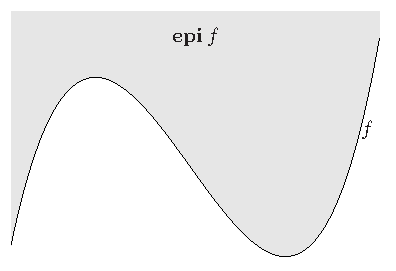
\includegraphics[width=.48\textwidth]{figures/ch03-90.pdf}
\caption*{图3.5 阴影部分是函数 $f$ 的上图。较深的下边界是 $f$ 的图像。}
\end{figure}
\begin{origexample}{3.4}
\textbf{矩阵分式函数。}函数 $f:\R^n\times\mathbb S^n\to\R$，
\[f(x,Y)=x^\T Y^{-1}x,\]
在 $\dom f=\R^n\times\mathbb S_{++}^n$ 上凸。（它推广了定义域为 $\R\times\R_{++}$ 的二次除以线性函数 $f(x,y)=x^2/y$。）

证明 $f$ 凸的一种简便方法是考察其上图：
\[
\begin{aligned}
 \epi f&=\{(x,Y,t)\mid Y\succ0,\ x^\T Y^{-1}x\leq t\}\\
 &=\left\{(x,Y,t)\ \middle|\
 \begin{bmatrix}Y&x\\x^\T&t\end{bmatrix}\succeq0,\ Y\succ0\right\}.
\end{aligned}
\]
这里使用了分块矩阵半正定的 Schur 补条件（见A.5.5节）。最后的条件是关于 $(x,Y,t)$ 的线性矩阵不等式，因此 $\epi f$ 凸。

在特殊情形 $n=1$ 下，矩阵分式函数成为二次除以线性函数 $x^2/y$，对应的 LMI 表示为
\[\begin{bmatrix}y&x\\x&t\end{bmatrix}\succeq0,\qquad y>0\]
（其函数图像见图3.3）。
\end{origexample}
凸函数的许多结论，都可以借助上图并应用凸集结论，从几何上证明或解释。例如，考虑凸性的一阶条件
\[f(y)\geq f(x)+\nabla f(x)^\T(y-x),\]
其中 $f$ 凸、$x,y\in\dom f$。这个基本不等式可以用 $\epi f$ 作几何解释。若 $(y,t)\in\epi f$，则
\[t\geq f(y)\geq f(x)+\nabla f(x)^\T(y-x).\]
% Source PDF page 91 (printed p. 77)
这可以写成
\[
 (y,t)\in\epi f\ \Longrightarrow\
 \begin{bmatrix}\nabla f(x)\\-1\end{bmatrix}^{\T}
 \left(\begin{bmatrix}y\\t\end{bmatrix}
 -\begin{bmatrix}x\\f(x)\end{bmatrix}\right)\leq0.
\]
这意味着，由 $(\nabla f(x),-1)$ 确定的超平面在边界点 $(x,f(x))$ 处支撑 $\epi f$；见图3.6。
\begin{figure}[htbp]\centering
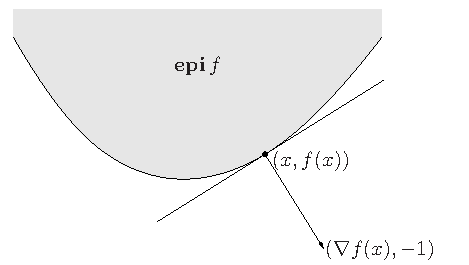
\includegraphics[width=.56\textwidth]{figures/ch03-91.pdf}
\caption*{图3.6 对可微凸函数 $f$，向量 $(\nabla f(x),-1)$ 确定了 $f$ 的上图在 $x$ 处的一个支撑超平面。}
\end{figure}
\subsection{Jensen 不等式及其推广}
基本不等式(3.1)，即
\[f(\theta x+(1-\theta)y)\leq\theta f(x)+(1-\theta)f(y),\]
有时称为 Jensen 不等式。它很容易推广到两个以上点的凸组合：若 $f$ 凸，$x_1,\ldots,x_k\in\dom f$，且 $\theta_1,\ldots,\theta_k\geq0$、$\theta_1+\cdots+\theta_k=1$，则
\[f(\theta_1x_1+\cdots+\theta_kx_k)\leq\theta_1f(x_1)+\cdots+\theta_kf(x_k).\]
如同凸集的情况，不等式还能推广到无穷和、积分与期望。例如，若 $p(x)\geq0$ 对 $S\subseteq\dom f$ 上的 $x$ 成立，且 $\int_S p(x)\,dx=1$，则
\[f\left(\int_S p(x)x\,dx\right)\leq\int_S f(x)p(x)\,dx,\]
只要这些积分存在。最一般的情况可以采用支撑位于 $\dom f$ 内的任意概率测度。若随机变量 $x$ 以概率一属于 $\dom f$，且 $f$ 凸，则
\begin{equation}f(\E x)\leq\E f(x),\tag{3.5}\end{equation}
只要这些期望存在。令随机变量 $x$ 的支撑为 $\{x_1,x_2\}$，且 $\Prob(x=x_1)=\theta$、$\Prob(x=x_2)=1-\theta$，就能从这一一般形式恢复基本不等式(3.1)。
% Source PDF page 92 (printed p. 78)
因此，不等式(3.5)刻画了凸性：若 $f$ 不凸，则存在一个以概率一属于 $\dom f$ 的随机变量 $x$，使 $f(\E x)>\E f(x)$。

现在，上述不等式都称为 Jensen 不等式，尽管 Jensen 研究的只是下面这个很简单的不等式：
\[f\left(\frac{x+y}2\right)\leq\frac{f(x)+f(y)}2.\]
\paragraph{注3.2}式(3.5)可以作如下解释。设 $x\in\dom f\subseteq\R^n$，$z$ 是 $\R^n$ 中任意零均值随机向量。则
\[\E f(x+z)\geq f(x).\]
因此，随机化或抖动（即在自变量上加一个零均值随机向量）不会使凸函数值的平均值降低。

\subsection{不等式}
对合适的凸函数应用 Jensen 不等式，可以导出许多著名不等式。（事实上，凸性与 Jensen 不等式可以作为不等式理论的基础。）举一个简单例子，考虑算术—几何平均不等式：对 $a,b\geq0$ 有
\begin{equation}\sqrt{ab}\leq(a+b)/2.\tag{3.6}\end{equation}
函数 $-\log x$ 凸，取 $\theta=1/2$ 应用 Jensen 不等式，得
\[-\log\frac{a+b}2\leq\frac{-\log a-\log b}2.\]
两边取指数，即得式(3.6)。

再看一个稍复杂的例子，证明 Hölder 不等式：对 $p>1$、$1/p+1/q=1$ 以及 $x,y\in\R^n$，有
\[
 \sum_{i=1}^n x_iy_i\leq
 \left(\sum_{i=1}^n|x_i|^p\right)^{1/p}
 \left(\sum_{i=1}^n|y_i|^q\right)^{1/q}.
\]
由 $-\log x$ 的凸性以及一般 $\theta$ 对应的 Jensen 不等式，得到更一般的算术—几何平均不等式
\[a^\theta b^{1-\theta}\leq\theta a+(1-\theta)b,\]
它对 $a,b\geq0$、$0\leq\theta\leq1$ 成立。取
\[a=\frac{|x_i|^p}{\sum_{j=1}^n|x_j|^p},\qquad
 b=\frac{|y_i|^q}{\sum_{j=1}^n|y_j|^q},\qquad\theta=1/p,\]
应用上述不等式，得
\[
 \left(\frac{|x_i|^p}{\sum_{j=1}^n|x_j|^p}\right)^{1/p}
 \left(\frac{|y_i|^q}{\sum_{j=1}^n|y_j|^q}\right)^{1/q}
 \leq\frac{|x_i|^p}{p\sum_{j=1}^n|x_j|^p}
       +\frac{|y_i|^q}{q\sum_{j=1}^n|y_j|^q}.
\]
再对 $i$ 求和，便得到 Hölder 不等式。
% Source PDF page 93 (printed p. 79)
\section{保持凸性的运算}
本节介绍一些保持函数凸性或凹性的运算，以及构造新凸函数和凹函数的方法。先从加法、数乘、逐点上确界等简单运算开始，再介绍更复杂的运算，其中一些包含前述简单运算作为特例。
\subsection{非负加权和}
显然，若 $f$ 为凸函数、$\alpha\geq0$，则 $\alpha f$ 凸。若 $f_1,f_2$ 都凸，则它们的和 $f_1+f_2$ 也凸。结合非负数乘和加法可知，凸函数的集合本身是一个凸锥：凸函数的非负加权和
\[f=w_1f_1+\cdots+w_mf_m\]
凸。类似地，凹函数的非负加权和凹。严格凸（凹）函数的非负、非零加权和严格凸（凹）。

这些性质可以推广到无穷和与积分。例如，若对每个 $y\in A$，$f(x,y)$ 关于 $x$ 凸，且 $w(y)\geq0$，则
\[g(x)=\int_A w(y)f(x,y)\,dy\]
关于 $x$ 凸，只要积分存在。

非负数乘和加法保持凸性，可以直接验证，也可以通过相应的上图看出。例如，若 $w\geq0$、$f$ 凸，则
\[\epi(wf)=\begin{bmatrix}I&0\\0&w\end{bmatrix}\epi f,\]
它是凸集，因为凸集在线性映射下的像凸。
\subsection{与仿射映射复合}
设 $f:\R^n\to\R$、$A\in\R^{n\times m}$、$b\in\R^n$。定义 $g:\R^m\to\R$ 为
\[g(x)=f(Ax+b),\]
定义域为 $\dom g=\{x\mid Ax+b\in\dom f\}$。若 $f$ 凸，则 $g$ 凸；若 $f$ 凹，则 $g$ 凹。
% Source PDF page 94 (printed p. 80)
\subsection{逐点最大值与上确界}
若 $f_1,f_2$ 是凸函数，则其逐点最大值
\[f(x)=\max\{f_1(x),f_2(x)\},\qquad\dom f=\dom f_1\cap\dom f_2\]
也凸。这个性质容易验证：若 $0\leq\theta\leq1$、$x,y\in\dom f$，则
\[
\begin{aligned}
 f(\theta x+(1-\theta)y)
 &=\max\{f_1(\theta x+(1-\theta)y),f_2(\theta x+(1-\theta)y)\}\\
 &\leq\max\{\theta f_1(x)+(1-\theta)f_1(y),\theta f_2(x)+(1-\theta)f_2(y)\}\\
 &\leq\theta\max\{f_1(x),f_2(x)\}+(1-\theta)\max\{f_1(y),f_2(y)\}\\
 &=\theta f(x)+(1-\theta)f(y),
\end{aligned}
\]
这证明了 $f$ 凸。也容易证明，若 $f_1,\ldots,f_m$ 凸，则它们的逐点最大值
\[f(x)=\max\{f_1(x),\ldots,f_m(x)\}\]
凸。
\begin{origexample}{3.5}
\textbf{分段线性函数。}函数
\[f(x)=\max\{a_1^\T x+b_1,\ldots,a_L^\T x+b_L\}\]
定义了一个至多有 $L$ 个区域的分段线性函数（严格说是分段仿射函数）。它凸，因为它是仿射函数的逐点最大值。

逆命题也可以证明：任何至多有 $L$ 个区域的分段线性凸函数，都可以表示成这种形式。（见习题3.29。）
\end{origexample}
\begin{origexample}{3.6}
\textbf{最大的 $r$ 个分量之和。}对于 $x\in\R^n$，用 $x_{[i]}$ 表示 $x$ 的第 $i$ 大分量，即
\[x_{[1]}\geq x_{[2]}\geq\cdots\geq x_{[n]}\]
是 $x$ 的分量按非增顺序排列后的结果。那么，函数
\[f(x)=\sum_{i=1}^r x_{[i]},\]
即 $x$ 中最大的 $r$ 个元素之和，是凸函数。把它写成
\[f(x)=\sum_{i=1}^r x_{[i]}
 =\max\{x_{i_1}+\cdots+x_{i_r}\mid1\leq i_1<i_2<\cdots<i_r\leq n\},\]
就能看出这一点：它是 $x$ 中任意 $r$ 个不同分量之和的最大值。由于它是 $n!/(r!(n-r)!)$ 个线性函数的逐点最大值，所以凸。

进一步可以证明，只要 $w_1\geq w_2\geq\cdots\geq w_r\geq0$，函数 $\sum_{i=1}^r w_i x_{[i]}$ 就凸。（见习题3.19。）
\end{origexample}
% Source PDF page 95 (printed p. 81)
逐点最大值的性质可以推广到无穷多个凸函数的逐点上确界。若对每个 $y\in A$，$f(x,y)$ 关于 $x$ 凸，则函数
\begin{equation}g(x)=\sup_{y\in A}f(x,y)\tag{3.7}\end{equation}
关于 $x$ 凸。这里 $g$ 的定义域是
\[\dom g=\{x\mid (x,y)\in\dom f\text{ 对所有 }y\in A\text{ 成立},\ \sup_{y\in A}f(x,y)<\infty\}.\]
类似地，一族凹函数的逐点下确界是凹函数。

从上图来看，函数的逐点上确界对应于上图的交。对式(3.7)定义的 $f,g,A$，有
\[\epi g=\bigcap_{y\in A}\epi f(\cdot,y).\]
因此，这一结论来自任意一族凸集的交仍凸。
\begin{origexample}{3.7}
\textbf{集合的支撑函数。}设 $C\subseteq\R^n$、$C\ne\varnothing$。与 $C$ 关联的支撑函数 $S_C$ 定义为
\[S_C(x)=\sup\{x^\T y\mid y\in C\},\]
自然有 $\dom S_C=\{x\mid\sup_{y\in C}x^\T y<\infty\}$。

对每个 $y\in C$，$x^\T y$ 是关于 $x$ 的线性函数，因此 $S_C$ 是一族线性函数的逐点上确界，从而凸。
\end{origexample}
\begin{origexample}{3.8}
\textbf{到集合最远点的距离。}设 $C\subseteq\R^n$。到 $C$ 中最远点的距离（采用任意范数）
\[f(x)=\sup_{y\in C}\norm{x-y}\]
凸。注意，对任意 $y$，$\norm{x-y}$ 关于 $x$ 凸。由于 $f$ 是一族以 $y\in C$ 为指标的凸函数的逐点上确界，所以它关于 $x$ 凸。
\end{origexample}
\begin{origexample}{3.9}
\textbf{最小二乘代价作为权重的函数。}设 $a_1,\ldots,a_n\in\R^m$。加权最小二乘问题是在 $x\in\R^m$ 上最小化目标 $\sum_{i=1}^n w_i(a_i^\T x-b_i)^2$。称 $w_i$ 为权重，允许它为负数（这使目标函数可能向下无界）。

定义最优加权最小二乘代价为
\[g(w)=\inf_x\sum_{i=1}^n w_i(a_i^\T x-b_i)^2,\]
其定义域为
\[\dom g=\left\{w\ \middle|\ \inf_x\sum_{i=1}^n w_i(a_i^\T x-b_i)^2>-\infty\right\}.\]
% Source PDF page 96 (printed p. 82)
由于 $g$ 是一族以 $x\in\R^m$ 为指标、关于 $w$ 的线性函数的下确界，所以关于 $w$ 凹。

至少在定义域的一部分上，可以导出 $g$ 的显式表达式。令 $W=\diag(w)$ 为对角元 $w_1,\ldots,w_n$ 组成的对角矩阵，$A\in\R^{n\times m}$ 的各行为 $a_i^\T$，于是
\[
 g(w)=\inf_x(Ax-b)^\T W(Ax-b)
 =\inf_x\bigl(x^\T A^\T WAx-2b^\T WAx+b^\T Wb\bigr).
\]
由此可见，若 $A^\T WA\not\succeq0$，这个关于 $x$ 的二次函数向下无界，因此 $g(w)=-\infty$，即 $w\notin\dom g$。当 $A^\T WA\succ0$（一个严格线性矩阵不等式）时，解析地最小化二次函数，就能给出 $g$ 的简单表达式：
\[
\begin{aligned}
 g(w)&=b^\T Wb-b^\T WA(A^\T WA)^{-1}A^\T Wb\\
 &=\sum_{i=1}^n w_i b_i^2-
 \sum_{i=1}^n w_i^2b_i^2a_i^\T
 \left(\sum_{j=1}^n w_ja_ja_j^\T\right)^{-1}a_i.
\end{aligned}
\]
从这个表达式不能立即看出 $g$ 的凹性，但可以由矩阵分式函数的凸性推出，例如见例3.4。
\end{origexample}
\begin{origexample}{3.10}
\textbf{对称矩阵的最大特征值。}函数 $f(X)=\lambda_{\max}(X)$、$\dom f=\mathbb S^m$ 凸，因为可以把它表示为
\[f(X)=\sup\{y^\T Xy\mid\norm y_2=1\},\]
即一族关于 $X$ 的线性函数 $y^\T Xy$ 的逐点上确界，其中以 $y\in\R^m$ 为指标。
\end{origexample}
\begin{origexample}{3.11}
\textbf{矩阵的范数。}考虑 $f(X)=\norm X_2$、$\dom f=\R^{p\times q}$，其中 $\norm{\cdot}_2$ 表示谱范数或最大奇异值。$f$ 的凸性来自
\[f(X)=\sup\{u^\T Xv\mid\norm u_2=1,\ \norm v_2=1\},\]
这表明它是一族关于 $X$ 的线性函数的逐点上确界。

推广这一结果，设 $\norm{\cdot}_a$、$\norm{\cdot}_b$ 分别是 $\R^p$ 和 $\R^q$ 上的范数。矩阵 $X\in\R^{p\times q}$ 的诱导范数定义为
\[\norm X_{a,b}=\sup_{v\ne0}\frac{\norm{Xv}_a}{\norm v_b}.\]
（当两个范数都是欧氏范数时，它就是谱范数。）诱导范数可以写为
\[
\begin{aligned}
 \norm X_{a,b}&=\sup\{\norm{Xv}_a\mid\norm v_b=1\}\\
 &=\sup\{u^\T Xv\mid\norm u_{a*}=1,\ \norm v_b=1\},
\end{aligned}
\]
其中 $\norm{\cdot}_{a*}$ 是 $\norm{\cdot}_a$ 的对偶范数，并使用了
\[\norm z_a=\sup\{u^\T z\mid\norm u_{a*}=1\}.\]
由于 $\norm X_{a,b}$ 已表示成关于 $X$ 的线性函数的上确界，它是凸函数。
\end{origexample}
% Source PDF page 97 (printed p. 83)
\subsubsection*{表示成仿射函数的逐点上确界}
上面的例子说明了一种证明函数凸性的好方法：把函数表示成一族仿射函数的逐点上确界。除一个技术条件外，逆命题也成立：几乎每个凸函数都能表示成一族仿射函数的逐点上确界。例如，若 $f:\R^n\to\R$ 凸，且 $\dom f=\R^n$，则
\[f(x)=\sup\{g(x)\mid g\text{ 仿射},\ g(z)\leq f(z)\text{ 对所有 }z\text{ 成立}\}.\]
换句话说，$f$ 是它的所有仿射全局下估计的逐点上确界。下面证明这一结论，$\dom f\ne\R^n$ 的情形留作习题3.28。

设 $f$ 凸，$\dom f=\R^n$。不等式
\[f(x)\geq\sup\{g(x)\mid g\text{ 仿射},\ g(z)\leq f(z)\text{ 对所有 }z\text{ 成立}\}\]
显然成立，因为 $f$ 的任意仿射下估计 $g$ 都有 $g(x)\leq f(x)$。为证明等号，我们将证明：对每个 $x\in\R^n$，都有一个 $f$ 的仿射全局下估计 $g$，满足 $g(x)=f(x)$。

$f$ 的上图当然是凸集。因此，在 $(x,f(x))$ 处能找到一个支撑超平面，即存在 $a\in\R^n$、$b\in\R$，$(a,b)\ne0$，且对所有 $(z,t)\in\epi f$ 有
\[\begin{bmatrix}a\\b\end{bmatrix}^{\T}
 \begin{bmatrix}x-z\\f(x)-t\end{bmatrix}\leq0.\]
这意味着，对所有 $z\in\dom f=\R^n$ 以及所有 $s\geq0$ 都有
\begin{equation}a^\T(x-z)+b(f(x)-f(z)-s)\leq0,\tag{3.8}\end{equation}
因为 $(z,t)\in\epi f$ 意味着存在 $s\geq0$ 使 $t=f(z)+s$。要使式(3.8)对所有 $s\geq0$ 成立，必须有 $b\geq0$。若 $b=0$，它就简化为对所有 $z\in\R^n$ 有 $a^\T(x-z)\leq0$，从而 $a=0$，这与 $(a,b)\ne0$ 矛盾。因此 $b>0$，即支撑超平面不竖直。

利用 $b>0$，取 $s=0$ 后将式(3.8)改写为
\[g(z)=f(x)+(a/b)^\T(x-z)\leq f(z)\qquad\text{对所有 }z.\]
函数 $g$ 是 $f$ 的仿射下估计，并满足 $g(x)=f(x)$。
\subsection{复合}
本节研究 $h:\R^k\to\R$ 与 $g:\R^n\to\R^k$ 应满足什么条件，才能保证它们的复合函数 $f=h\circ g:\R^n\to\R$ 凸或凹。其中
\[f(x)=h(g(x)),\qquad\dom f=\{x\in\dom g\mid g(x)\in\dom h\}.\]
% Source PDF page 98 (printed p. 84)
\subsubsection*{标量复合}
先考虑 $k=1$，即 $h:\R\to\R$、$g:\R^n\to\R$。只需讨论 $n=1$，因为凸性由函数在任意与定义域相交的直线上的表现决定。

为发现复合规则，先假设 $h,g$ 二次可微，且 $\dom g=\dom h=\R$。此时 $f$ 凸等价于 $f''\geq0$（即对所有 $x\in\R$ 有 $f''(x)\geq0$）。复合函数 $f=h\circ g$ 的二阶导数为
\begin{equation}f''(x)=h''(g(x))g'(x)^2+h'(g(x))g''(x).\tag{3.9}\end{equation}
例如，设 $g$ 凸（所以 $g''\geq0$），$h$ 凸且单调不减（所以 $h''\geq0$、$h'\geq0$）。由式(3.9)有 $f''\geq0$，即 $f$ 凸。类似地，式(3.9)给出以下结论：
\begin{equation}
\begin{array}{ll}
 f\text{ 凸，若 }h\text{ 凸且单调不减，}g\text{ 凸；}\\
 f\text{ 凸，若 }h\text{ 凸且单调不增，}g\text{ 凹；}\\
 f\text{ 凹，若 }h\text{ 凹且单调不减，}g\text{ 凹；}\\
 f\text{ 凹，若 }h\text{ 凹且单调不增，}g\text{ 凸。}
\end{array}\tag{3.10}
\end{equation}
这些命题在 $g,h$ 二次可微、定义域都是整个 $\R$ 时成立。事实上，在一般的 $n>1$ 情况下，不要求 $h,g$ 可微，也不要求 $\dom g=\R^n$、$\dom h=\R$，仍有非常类似的复合规则：
\begin{equation}
\begin{array}{ll}
 f\text{ 凸，若 }h\text{ 凸，}\widetilde h\text{ 单调不减，}g\text{ 凸；}\\
 f\text{ 凸，若 }h\text{ 凸，}\widetilde h\text{ 单调不增，}g\text{ 凹；}\\
 f\text{ 凹，若 }h\text{ 凹，}\widetilde h\text{ 单调不减，}g\text{ 凹；}\\
 f\text{ 凹，若 }h\text{ 凹，}\widetilde h\text{ 单调不增，}g\text{ 凸。}
\end{array}\tag{3.11}
\end{equation}
这里 $\widetilde h$ 表示函数 $h$ 的扩展值延拓：当 $h$ 凸（凹）时，它在不属于 $\dom h$ 的点取 $\infty$（$-\infty$）。这些结论与式(3.10)唯一的差别，是要求扩展值延拓 $\widetilde h$ 在整个 $\R$ 上单调不增或单调不减。

为理解其含义，设 $h$ 凸，则 $\widetilde h$ 在 $\dom h$ 外取值 $\infty$。$\widetilde h$ 单调不减意味着，对任意 $x,y\in\R$、$x<y$，有 $\widetilde h(x)\leq\widetilde h(y)$。特别地，这意味着若 $y\in\dom h$，则 $x\in\dom h$。换句话说，$h$ 的定义域沿负方向无限延伸：它或者是 $\R$，或者是 $(-\infty,a)$、$(-\infty,a]$ 形式的区间。类似地，$h$ 凸且 $\widetilde h$ 单调不增，意味着 $h$ 单调不增，且 $\dom h$ 沿正方向无限延伸。图3.7说明了这一点。
\begin{origexample}{3.12}
下面几个简单例子说明复合定理中关于 $h$ 的条件。
\begin{itemize}
\item 函数 $h(x)=\log x$，$\dom h=\R_{++}$，凹且 $\widetilde h$ 单调不减。
% Source PDF page 99 (printed p. 85)
\item 函数 $h(x)=x^{1/2}$、$\dom h=\R_+$，凹且满足 $\widetilde h$ 单调不减。
\item 函数 $h(x)=x^{3/2}$、$\dom h=\R_+$，凸，但不满足 $\widetilde h$ 单调不减。例如，$\widetilde h(-1)=\infty$，而 $\widetilde h(1)=1$。
\item 定义域为 $\R$、在 $x\geq0$ 时 $h(x)=x^{3/2}$、在 $x<0$ 时 $h(x)=0$ 的函数凸，并满足 $\widetilde h$ 单调不减。
\end{itemize}
\end{origexample}
\begin{figure}[htbp]\centering
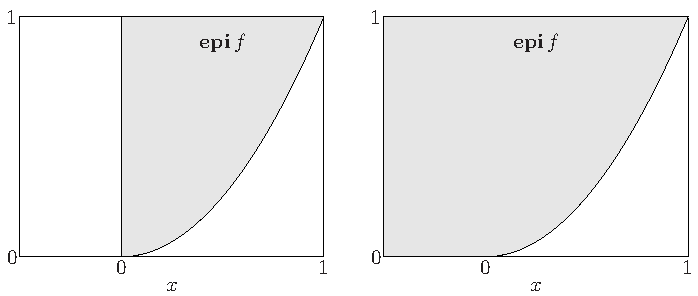
\includegraphics[width=.75\textwidth]{figures/ch03-99.pdf}
\caption*{图3.7 左：定义域为 $\R_+$ 的函数 $x^2$ 凸且在定义域上单调不减，但其扩展值延拓并不单调不减。右：定义域为 $\R$ 的函数 $\max\{x,0\}^2$ 凸，且其扩展值延拓单调不减。}
\end{figure}
复合结论(3.11)可以直接证明，不必假设可微，也不必使用公式(3.9)。例如，证明如下复合定理：若 $g$ 凸、$h$ 凸且 $\widetilde h$ 单调不减，则 $f=h\circ g$ 凸。设 $x,y\in\dom f$、$0\leq\theta\leq1$。由 $x,y\in\dom f$，有 $x,y\in\dom g$ 以及 $g(x),g(y)\in\dom h$。由于 $\dom g$ 凸，有 $\theta x+(1-\theta)y\in\dom g$，再由 $g$ 的凸性得
\begin{equation}g(\theta x+(1-\theta)y)\leq\theta g(x)+(1-\theta)g(y).\tag{3.12}\end{equation}
因为 $g(x),g(y)\in\dom h$，所以 $\theta g(x)+(1-\theta)g(y)\in\dom h$，即式(3.12)右端属于 $\dom h$。现在使用 $\widetilde h$ 单调不减这一假设，它意味着定义域沿负方向无限延伸。式(3.12)右端属于 $\dom h$，故左端 $g(\theta x+(1-\theta)y)$ 也属于 $\dom h$。这意味着 $\theta x+(1-\theta)y\in\dom f$。至此已证明 $\dom f$ 凸。

再利用 $\widetilde h$ 单调不减和不等式(3.12)，得
\begin{equation}h(g(\theta x+(1-\theta)y))\leq h(\theta g(x)+(1-\theta)g(y)).\tag{3.13}\end{equation}
由 $h$ 的凸性有
\begin{equation}h(\theta g(x)+(1-\theta)g(y))\leq\theta h(g(x))+(1-\theta)h(g(y)).\tag{3.14}\end{equation}
% Source PDF page 100 (printed p. 86)
合并式(3.13)与(3.14)，得到
\[h(g(\theta x+(1-\theta)y))\leq\theta h(g(x))+(1-\theta)h(g(y)),\]
从而证明了复合定理。
\begin{origexample}{3.13}
\textbf{简单的复合结论。}
\begin{itemize}
\item 若 $g$ 凸，则 $\exp g(x)$ 凸。
\item 若 $g$ 凹且为正，则 $\log g(x)$ 凹。
\item 若 $g$ 凹且为正，则 $1/g(x)$ 凸。
\item 若 $g$ 凸且非负、$p\geq1$，则 $g(x)^p$ 凸。
\item 若 $g$ 凸，则 $-\log(-g(x))$ 在 $\{x\mid g(x)<0\}$ 上凸。
\end{itemize}
\end{origexample}
\paragraph{注3.3}不能把扩展值延拓 $\widetilde h$ 的单调性要求，放宽为只要求函数 $h$ 单调。例如，考虑 $g(x)=x^2$、$\dom g=\R$，以及 $h(x)=0$、$\dom h=[1,2]$。这里 $g$ 凸，$h$ 凸且单调不减，但复合函数 $f=h\circ g$，即
\[f(x)=0,\qquad\dom f=[-\sqrt2,-1]\cup[1,\sqrt2],\]
不凸，因为定义域不凸。这里的 $\widetilde h$ 当然并不单调不减。

\subsubsection*{向量复合}
现在考虑更复杂的 $k\geq1$ 情形。设
\[f(x)=h(g(x))=h(g_1(x),\ldots,g_k(x)),\]
其中 $h:\R^k\to\R$、$g_i:\R^n\to\R$。仍可不失一般性地假设 $n=1$。如同 $k=1$，为发现复合规则，先假设函数二次可微，且 $\dom g=\R$、$\dom h=\R^k$。有
\begin{equation}
 f''(x)=g'(x)^\T\nabla^2h(g(x))g'(x)+\nabla h(g(x))^\T g''(x),\tag{3.15}
\end{equation}
这是式(3.9)的向量形式。问题仍是确定哪些条件可以保证对所有 $x$ 有 $f''(x)\geq0$（凹性则对应 $f''(x)\leq0$）。由式(3.15)可以导出许多规则，例如：
\begin{itemize}
\item 若 $h$ 凸、对每个自变量单调不减，且各 $g_i$ 凸，则 $f$ 凸；
\item 若 $h$ 凸、对每个自变量单调不增，且各 $g_i$ 凹，则 $f$ 凸；
\item 若 $h$ 凹、对每个自变量单调不减，且各 $g_i$ 凹，则 $f$ 凹。
\end{itemize}
% Source PDF page 101 (printed p. 87)
与标量情况一样，在 $n>1$、不假设 $h,g$ 可微、定义域一般的情况下，类似的复合结论仍成立。一般结论要求 $h$ 的单调性条件对扩展值延拓 $\widetilde h$ 成立。

为理解扩展值延拓 $\widetilde h$ 的单调性条件，考虑 $h:\R^k\to\R$ 凸，$\widetilde h$ 单调不减的情况，即只要 $u\preceq v$ 就有 $\widetilde h(u)\leq\widetilde h(v)$。这意味着，若 $v\in\dom h$，则 $u\in\dom h$：$h$ 的定义域必须沿 $-\R_+^k$ 的方向无限延伸。可以简写为 $\dom h-\R_+^k=\dom h$。
\begin{origexample}{3.14}
\textbf{向量复合的例子。}
\begin{itemize}
\item 令 $h(z)=z_{[1]}+\cdots+z_{[r]}$，即 $z\in\R^k$ 中最大的 $r$ 个分量之和。$h$ 凸且对每个自变量单调不减。设 $g_1,\ldots,g_k$ 是 $\R^n$ 上的凸函数，则复合函数 $f=h\circ g$，也就是各 $g_i$ 中最大的 $r$ 个的逐点和，凸。
\item 函数 $h(z)=\log(\sum_{i=1}^k e^{z_i})$ 凸且对每个自变量单调不减，因此只要各 $g_i$ 凸，$\log(\sum_{i=1}^k e^{g_i})$ 就凸。
\item 对 $0<p\leq1$，函数 $h(z)=(\sum_{i=1}^k z_i^p)^{1/p}$ 在 $\R_+^k$ 上凹，且其延拓（在 $z\not\succeq0$ 时取 $-\infty$）对每个分量单调不减。因此，若各 $g_i$ 凹且非负，则 $f(x)=(\sum_{i=1}^k g_i(x)^p)^{1/p}$ 凹。
\item 设 $p\geq1$，$g_1,\ldots,g_k$ 凸且非负，则函数 $(\sum_{i=1}^k g_i(x)^p)^{1/p}$ 凸。为证明这一点，考虑 $h:\R^k\to\R$，
\[h(z)=\left(\sum_{i=1}^k\max\{z_i,0\}^p\right)^{1/p},\]
其中 $\dom h=\R^k$，所以 $h=\widetilde h$。此函数凸且单调不减，故 $h(g(x))$ 关于 $x$ 凸。对 $z\succeq0$，$h(z)=(\sum_{i=1}^k z_i^p)^{1/p}$，于是得到 $(\sum_{i=1}^k g_i(x)^p)^{1/p}$ 凸。
\item 几何平均 $h(z)=(\prod_{i=1}^k z_i)^{1/k}$ 在 $\R_+^k$ 上凹，且其延拓对每个自变量单调不减。因此，若 $g_1,\ldots,g_k$ 是非负凹函数，它们的几何平均 $(\prod_{i=1}^k g_i)^{1/k}$ 也凹。
\end{itemize}
\end{origexample}
\subsection{最小化}
我们已经看到，任意一族凸函数的最大值或上确界凸。事实上，某些特殊形式的最小化也能产生凸函数。若 $f$ 关于 $(x,y)$ 凸，且 $C$ 为非空凸集，则函数
\begin{equation}g(x)=\inf_{y\in C}f(x,y)\tag{3.16}\end{equation}
% Source PDF page 102 (printed p. 88)
关于 $x$ 凸，只要对所有 $x$ 都有 $g(x)>-\infty$。$g$ 的定义域是 $\dom f$ 在 $x$ 坐标上的投影，即
\[\dom g=\{x\mid\text{存在 }y\in C\text{ 使 }(x,y)\in\dom f\}.\]
下面对 $x_1,x_2\in\dom g$ 验证 Jensen 不等式，证明这一结论。令 $\epsilon>0$。存在 $y_1,y_2\in C$，使 $f(x_i,y_i)\leq g(x_i)+\epsilon$，$i=1,2$。再令 $\theta\in[0,1]$，有
\[
\begin{aligned}
 g(\theta x_1+(1-\theta)x_2)
 &=\inf_{y\in C}f(\theta x_1+(1-\theta)x_2,y)\\
 &\leq f(\theta x_1+(1-\theta)x_2,\theta y_1+(1-\theta)y_2)\\
 &\leq\theta f(x_1,y_1)+(1-\theta)f(x_2,y_2)\\
 &\leq\theta g(x_1)+(1-\theta)g(x_2)+\epsilon.
\end{aligned}
\]
由于这对任意 $\epsilon>0$ 成立，得到
\[g(\theta x_1+(1-\theta)x_2)\leq\theta g(x_1)+(1-\theta)g(x_2).\]
这一结论也可以通过上图看出。$f,g,C$ 如式(3.16)所定义，并假设每个 $x$ 处对 $y\in C$ 的下确界都能取到，则
\[\epi g=\{(x,t)\mid\text{存在 }y\in C\text{ 使 }(x,y,t)\in\epi f\}.\]
因此 $\epi g$ 凸，因为它是凸集在部分坐标上的投影。
\begin{origexample}{3.15}
\textbf{Schur 补。}设二次函数
\[f(x,y)=x^\T Ax+2x^\T By+y^\T Cy,\]
其中 $A,C$ 对称，关于 $(x,y)$ 凸，这意味着
\[\begin{bmatrix}A&B\\B^\T&C\end{bmatrix}\succeq0.\]
可以将 $g(x)=\inf_y f(x,y)$ 表示为
\[g(x)=x^\T(A-BC^\dagger B^\T)x,\]
其中 $C^\dagger$ 是 $C$ 的伪逆（见A.5.4节）。由最小化规则，$g$ 凸，因此 $A-BC^\dagger B^\T\succeq0$。

若 $C$ 可逆，即 $C\succ0$，则矩阵 $A-BC^{-1}B^\T$ 称为 $C$ 在矩阵
\[\begin{bmatrix}A&B\\B^\T&C\end{bmatrix}\]
中的 Schur 补（见A.5.5节）。
\end{origexample}
\begin{origexample}{3.16}
\textbf{到集合的距离。}在范数 $\norm{\cdot}$ 下，点 $x$ 到集合 $S\subseteq\R^n$ 的距离定义为
\[\dist(x,S)=\inf_{y\in S}\norm{x-y}.\]
函数 $\norm{x-y}$ 关于 $(x,y)$ 凸，因此若 $S$ 凸，则距离函数 $\dist(x,S)$ 关于 $x$ 凸。
\end{origexample}
% Source PDF page 103 (printed p. 89)
\begin{origexample}{3.17}
设 $h$ 凸，则函数
\[g(x)=\inf\{h(y)\mid Ay=x\}\]
凸。为证明这一点，定义
\[f(x,y)=\begin{cases}h(y),&Ay=x,\\\infty,&\text{其他情况},\end{cases}\]
它关于 $(x,y)$ 凸。$g$ 是 $f$ 对 $y$ 的最小值，因此凸。（直接证明 $g$ 凸也并不难。）
\end{origexample}
\subsection{函数的透视}
若 $f:\R^n\to\R$，则 $f$ 的透视是函数 $g:\R^{n+1}\to\R$，定义为
\[g(x,t)=tf(x/t),\]
定义域为
\[\dom g=\{(x,t)\mid x/t\in\dom f,\ t>0\}.\]
透视运算保持凸性：若 $f$ 凸，其透视函数 $g$ 也凸。类似地，若 $f$ 凹，则 $g$ 凹。

这一结论有多种证明，例如直接验证定义不等式（见习题3.33）。这里用上图和2.3.3节介绍的 $\R^{n+1}$ 上的透视映射，给出简短证明，这也解释了“透视”一词的由来。对 $t>0$ 有
\[
\begin{aligned}
 (x,t,s)\in\epi g&\Longleftrightarrow tf(x/t)\leq s\\
 &\Longleftrightarrow f(x/t)\leq s/t\\
 &\Longleftrightarrow(x/t,s/t)\in\epi f.
\end{aligned}
\]
因此，$\epi g$ 是 $\epi f$ 在将 $(u,v,w)$ 映到 $(u,w)/v$ 的透视映射下的逆像。由2.3.3节，$\epi g$ 凸，故 $g$ 凸。
\begin{origexample}{3.18}
\textbf{欧氏范数的平方。}$\R^n$ 上凸函数 $f(x)=x^\T x$ 的透视为
\[g(x,t)=t(x/t)^\T(x/t)=\frac{x^\T x}{t},\]
当 $t>0$ 时关于 $(x,t)$ 凸。

也可以用几种其他方法推出 $g$ 凸。首先，将 $g$ 写成二次除以线性函数 $x_i^2/t$ 的和，这些函数已在3.1.5节证明为凸。也可以将 $g$ 表示为矩阵分式函数的特例 $x^\T(tI)^{-1}x$（见例3.4）。
\end{origexample}
% Source PDF page 104 (printed p. 90)
\begin{origexample}{3.19}
\textbf{负对数。}考虑 $\R_{++}$ 上的凸函数 $f(x)=-\log x$。它的透视为
\[g(x,t)=-t\log(x/t)=t\log(t/x)=t\log t-t\log x,\]
在 $\R_{++}^2$ 上凸。函数 $g$ 称为 $t$ 和 $x$ 的相对熵。当 $x=1$ 时，$g$ 成为负熵函数。

从 $g$ 的凸性可以证明几个相关函数的凸性或凹性。首先，两个向量 $u,v\in\R_{++}^n$ 的相对熵定义为
\[\sum_{i=1}^n u_i\log(u_i/v_i),\]
它关于 $(u,v)$ 凸，因为它是各对 $u_i,v_i$ 相对熵之和。

一个密切相关的函数是 $u,v\in\R_{++}^n$ 之间的 Kullback--Leibler 散度，
\begin{equation}
 D_{\mathrm{kl}}(u,v)=\sum_{i=1}^n\bigl(u_i\log(u_i/v_i)-u_i+v_i\bigr),\tag{3.17}
\end{equation}
它凸，因为它是相对熵加上 $(u,v)$ 的线性函数。Kullback--Leibler 散度满足 $D_{\mathrm{kl}}(u,v)\geq0$，且 $D_{\mathrm{kl}}(u,v)=0$ 当且仅当 $u=v$，因此可用来度量两个正向量之间的偏离程度；见习题3.13。（当 $u,v$ 为概率向量，即 $\one^\T u=\one^\T v=1$ 时，相对熵与 Kullback--Leibler 散度相同。）

在相对熵函数中取 $v_i=\one^\T u$，便得到 $u\in\R_{++}^n$ 的凹函数，而且具有齐次性：
\[\sum_{i=1}^n u_i\log(\one^\T u/u_i)=(\one^\T u)\sum_{i=1}^n z_i\log(1/z_i),\]
其中 $z=u/(\one^\T u)$，该函数称为归一化熵函数。向量 $z=u/(\one^\T u)$ 的分量和为一，是归一化向量或概率分布；$u$ 的归一化熵是此归一化分布的熵乘以 $\one^\T u$。
\end{origexample}
\begin{origexample}{3.20}
设 $f:\R^m\to\R$ 凸，$A\in\R^{m\times n}$、$b\in\R^m$、$c\in\R^n$、$d\in\R$。定义
\[g(x)=(c^\T x+d)f\bigl((Ax+b)/(c^\T x+d)\bigr),\]
定义域为
\[\dom g=\{x\mid c^\T x+d>0,\ (Ax+b)/(c^\T x+d)\in\dom f\}.\]
则 $g$ 凸。
\end{origexample}
\section{共轭函数}
本节介绍一种将在后面章节起重要作用的运算。
% Source PDF page 105 (printed p. 91)
\begin{figure}[htbp]\centering
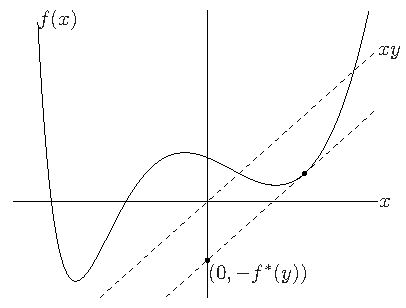
\includegraphics[width=.5\textwidth]{figures/ch03-105.pdf}
\caption*{图3.8 函数 $f:\R\to\R$ 以及一个数 $y\in\R$。共轭函数 $f^*(y)$ 是线性函数 $yx$ 与 $f(x)$ 之间的最大差距，由图中的虚线表示。若 $f$ 可微，这个最大差距在满足 $f'(x)=y$ 的点 $x$ 处取得。}
\end{figure}
\subsection{定义与例子}
设 $f:\R^n\to\R$。函数 $f^*:\R^n\to\R$，
\begin{equation}f^*(y)=\sup_{x\in\dom f}\bigl(y^\T x-f(x)\bigr),\tag{3.18}\end{equation}
称为 $f$ 的共轭函数。其定义域由使上确界有限的 $y\in\R^n$ 组成，即差 $y^\T x-f(x)$ 在 $\dom f$ 上有上界的那些 $y$。图3.8说明了这一定义。

可以立即看出，$f^*$ 凸，因为它是一族关于 $y$ 的凸函数（事实上为仿射函数）的逐点上确界。不论 $f$ 是否凸，这都成立。（当 $f$ 凸时，不必写出下标 $x\in\dom f$，因为按约定，对 $x\notin\dom f$ 有 $y^\T x-f(x)=-\infty$。）

先给出几个简单例子，再介绍一些求函数共轭的规则。这样就能导出许多常见凸函数的共轭函数的解析表达式。
\begin{origexample}{3.21}
下面求出 $\R$ 上几个凸函数的共轭。
\begin{itemize}
\item \textbf{仿射函数。}$f(x)=ax+b$。作为 $x$ 的函数，$yx-ax-b$ 有界当且仅当 $y=a$，此时它是常数。因此共轭函数 $f^*$ 的定义域为单点集 $\{a\}$，且 $f^*(a)=-b$。
\item \textbf{负对数。}$f(x)=-\log x$、$\dom f=\R_{++}$。若 $y\geq0$，函数 $xy+\log x$ 向上无界；否则在 $x=-1/y$ 处取得最大值。因此，$\dom f^*=\{y\mid y<0\}=-\R_{++}$，且对 $y<0$ 有 $f^*(y)=-\log(-y)-1$。
\item \textbf{指数。}$f(x)=e^x$。若 $y<0$，$xy-e^x$ 无界。若 $y>0$，$xy-e^x$ 在 $x=\log y$ 处取得最大值，所以 $f^*(y)=y\log y-y$。当 $y=0$ 时，
% Source PDF page 106 (printed p. 92)
$f^*(y)=\sup_x(-e^x)=0$。综上，$\dom f^*=\R_+$，$f^*(y)=y\log y-y$，其中约定 $0\log0=0$。
\item \textbf{负熵。}$f(x)=x\log x$、$\dom f=\R_+$，并令 $f(0)=0$。对所有 $y$，函数 $xy-x\log x$ 在 $\R_+$ 上有上界，因此 $\dom f^*=\R$。它在 $x=e^{y-1}$ 处取得最大值，代入得到 $f^*(y)=e^{y-1}$。
\item \textbf{倒数。}$f(x)=1/x$，定义在 $\R_{++}$ 上。当 $y>0$ 时，$yx-1/x$ 向上无界；当 $y=0$ 时，上确界为零；当 $y<0$ 时，在 $x=(-y)^{-1/2}$ 处取得上确界。因此，$f^*(y)=-2(-y)^{1/2}$，$\dom f^*=-\R_+$。
\end{itemize}
\end{origexample}
\begin{origexample}{3.22}
\textbf{严格凸二次函数。}考虑 $f(x)=\tfrac12x^\T Qx$，$Q\in\mathbb S_{++}^n$。对所有 $y$，关于 $x$ 的函数 $y^\T x-\tfrac12x^\T Qx$ 都有上界。它在 $x=Q^{-1}y$ 处取得最大值，故
\[f^*(y)=\tfrac12y^\T Q^{-1}y.\]
\end{origexample}
\begin{origexample}{3.23}
\textbf{行列式的对数。}考虑 $\mathbb S_{++}^n$ 上的 $f(X)=\log\det X^{-1}$。共轭函数定义为
\[f^*(Y)=\sup_{X\succ0}\bigl(\tr(YX)+\log\det X\bigr),\]
因为 $\tr(YX)$ 是 $\mathbb S^n$ 上的标准内积。先证明，除非 $Y\prec0$，否则 $\tr(YX)+\log\det X$ 向上无界。若 $Y\not\prec0$，则 $Y$ 有一个特征向量 $v$，满足 $\norm v_2=1$，对应特征值 $\lambda\geq0$。取 $X=I+tvv^\T$，则
\[
 \tr(YX)+\log\det X=\tr Y+t\lambda+\log\det(I+tvv^\T)
 =\tr Y+t\lambda+\log(1+t),
\]
当 $t\to\infty$ 时向上无界。

再考虑 $Y\prec0$。令关于 $X$ 的梯度为零，可以找到使目标最大的 $X$：
\[\nabla_X\bigl(\tr(YX)+\log\det X\bigr)=Y+X^{-1}=0\]
（见A.4.1节），得到 $X=-Y^{-1}$，它确实正定。因此
\[f^*(Y)=\log\det(-Y)^{-1}-n,\qquad\dom f^*=-\mathbb S_{++}^n.\]
\end{origexample}
\begin{origexample}{3.24}
\textbf{示性函数。}设 $I_S$ 为集合 $S\subseteq\R^n$（不一定凸）的示性函数，即 $I_S(x)=0$，$\dom I_S=S$。它的共轭为
\[I_S^*(y)=\sup_{x\in S}y^\T x,\]
即集合 $S$ 的支撑函数。
\end{origexample}
% Source PDF page 107 (printed p. 93)
\begin{origexample}{3.25}
\textbf{指数和对数函数。}为求 $f(x)=\log(\sum_{i=1}^n e^{x_i})$ 的共轭，先确定哪些 $y$ 能使 $y^\T x-f(x)$ 关于 $x$ 的最大值取到。令关于 $x$ 的梯度为零，得到条件
\[y_i=\frac{e^{x_i}}{\sum_{j=1}^n e^{x_j}},\qquad i=1,\ldots,n.\]
这些方程关于 $x$ 有解，当且仅当 $y\succ0$ 且 $\one^\T y=1$。把 $y_i$ 的表达式代入 $y^\T x-f(x)$，得到 $f^*(y)=\sum_{i=1}^n y_i\log y_i$。即使 $y$ 的某些分量为零，只要 $y\succeq0$、$\one^\T y=1$，并约定 $0\log0=0$，这个表达式仍成立。

事实上，$f^*$ 的定义域恰由 $\one^\T y=1$、$y\succeq0$ 给出。为证明这一点，先设 $y$ 有一个负分量，例如 $y_k<0$。取 $x_k=-t$、$x_i=0$（$i\ne k$），再令 $t\to\infty$，就能证明 $y^\T x-f(x)$ 向上无界。若 $y\succeq0$ 但 $\one^\T y\ne1$，取 $x=t\one$，有
\[y^\T x-f(x)=t\one^\T y-t-\log n.\]
若 $\one^\T y>1$，它在 $t\to\infty$ 时无界增大；若 $\one^\T y<1$，则在 $t\to-\infty$ 时无界增大。

综上，
\[f^*(y)=\begin{cases}\sum_{i=1}^n y_i\log y_i,&y\succeq0,\ \one^\T y=1,\\
 \infty,&\text{其他情况}.\end{cases}\]
换句话说，指数和对数函数的共轭，是限制在概率单纯形上的负熵函数。
\end{origexample}
\begin{origexample}{3.26}
\textbf{范数。}设 $\norm{\cdot}$ 是 $\R^n$ 上的范数，对偶范数为 $\norm{\cdot}_*$。将证明，$f(x)=\norm x$ 的共轭为
\[f^*(y)=\begin{cases}0,&\norm y_*\leq1,\\\infty,&\text{其他情况},\end{cases}\]
即范数的共轭是对偶范数单位球的示性函数。

若 $\norm y_*>1$，则由对偶范数定义，存在 $z\in\R^n$，$\norm z\leq1$，使 $y^\T z>1$。取 $x=tz$ 并令 $t\to\infty$，有
\[y^\T x-\norm x=t(y^\T z-\norm z)\to\infty,\]
表明 $f^*(y)=\infty$。反过来，若 $\norm y_*\leq1$，则对所有 $x$ 有 $y^\T x\leq\norm x\norm y_*$，从而 $y^\T x-\norm x\leq0$。因此，$x=0$ 使 $y^\T x-\norm x$ 达到最大值零。
\end{origexample}
\begin{origexample}{3.27}
\textbf{范数的平方。}现在考虑 $f(x)=\tfrac12\norm x^2$，其中 $\norm{\cdot}$ 为范数，对偶范数为 $\norm{\cdot}_*$。将证明其共轭为 $f^*(y)=\tfrac12\norm y_*^2$。由 $y^\T x\leq\norm y_*\norm x$ 得
\[y^\T x-\tfrac12\norm x^2\leq\norm y_*\norm x-\tfrac12\norm x^2\]
% Source PDF page 108 (printed p. 94)
对所有 $x$ 成立。右端是关于 $\norm x$ 的二次函数，最大值为 $\tfrac12\norm y_*^2$。因此对所有 $x$ 都有
\[y^\T x-\tfrac12\norm x^2\leq\tfrac12\norm y_*^2,\]
表明 $f^*(y)\leq\tfrac12\norm y_*^2$。

为证明另一个方向，取满足 $y^\T x=\norm y_*\norm x$ 的任意向量 $x$，并缩放至 $\norm x=\norm y_*$。对这个 $x$ 有
\[y^\T x-\tfrac12\norm x^2=\tfrac12\norm y_*^2,\]
表明 $f^*(y)\geq\tfrac12\norm y_*^2$。
\end{origexample}
\begin{origexample}{3.28}
\textbf{收入与利润函数。}考虑一家消耗 $n$ 种资源、生产可供销售产品的企业。用 $r=(r_1,\ldots,r_n)$ 表示消耗的资源数量向量，用 $S(r)$ 表示产品带来的销售收入，它是所耗资源的函数。令 $p_i$ 为第 $i$ 种资源的单位价格，则企业为资源支付的总金额为 $p^\T r$，利润为 $S(r)-p^\T r$。固定资源价格，问：通过合理选择消耗的资源数量，最多能获得多少利润？最大利润为
\[M(p)=\sup_r\bigl(S(r)-p^\T r\bigr).\]
函数 $M(p)$ 给出可达到的最大利润，作为资源价格的函数。用共轭函数可以写成
\[M(p)=(-S)^*(-p).\]
因此，最大利润（资源价格的函数）与销售总收入（所耗资源的函数）的共轭密切相关。
\end{origexample}
\subsection{基本性质}
\subsubsection*{Fenchel 不等式}
由共轭函数的定义，立即得到对所有 $x,y$ 成立的不等式
\[f(x)+f^*(y)\geq x^\T y.\]
它称为 Fenchel 不等式（当 $f$ 可微时，也称 Young 不等式）。

例如，对 $f(x)=\tfrac12x^\T Qx$、$Q\in\mathbb S_{++}^n$，得到
\[x^\T y\leq\tfrac12x^\T Qx+\tfrac12y^\T Q^{-1}y.\]
\subsubsection*{共轭的共轭}
上述例子以及“共轭”这个名称，都暗示凸函数的共轭的共轭就是原函数。满足一个技术条件时确实如此：若 $f$ 凸且闭（即 $\epi f$ 为闭集；见A.3.3节），则 $f^{**}=f$。例如，若 $\dom f=\R^n$，就有 $f^{**}=f$，即 $f$ 的共轭的共轭仍为 $f$（见习题3.39）。
% Source PDF page 109 (printed p. 95)
\subsubsection*{可微函数}
可微函数 $f$ 的共轭也称为 $f$ 的 Legendre 变换。（为区别一般定义与可微情形，有时用 Fenchel 共轭一词代替共轭。）

设 $f$ 凸且可微，$\dom f=\R^n$。使 $y^\T x-f(x)$ 最大的任意 $x^*$ 都满足 $y=\nabla f(x^*)$；反过来，若 $x^*$ 满足 $y=\nabla f(x^*)$，则 $x^*$ 使 $y^\T x-f(x)$ 最大。因此，当 $y=\nabla f(x^*)$ 时，
\[f^*(y)=x^{*\T}\nabla f(x^*)-f(x^*).\]
因此，只要对给定 $y$ 能解出梯度方程 $y=\nabla f(z)$ 中的 $z$，就能确定 $f^*(y)$。

也可以换一种表达方式：任取 $z\in\R^n$，定义 $y=\nabla f(z)$，则
\[f^*(y)=z^\T\nabla f(z)-f(z).\]
\subsubsection*{数乘及与仿射变换复合}
对 $a>0$、$b\in\R$，$g(x)=af(x)+b$ 的共轭为 $g^*(y)=af^*(y/a)-b$。

设 $A\in\R^{n\times n}$ 非奇异，$b\in\R^n$。则 $g(x)=f(Ax+b)$ 的共轭为
\[g^*(y)=f^*(A^{-\T}y)-b^\T A^{-\T}y,\qquad\dom g^*=A^\T\dom f^*.\]
\subsubsection*{相互独立函数之和}
若 $f(u,v)=f_1(u)+f_2(v)$，其中 $f_1,f_2$ 为凸函数，共轭分别为 $f_1^*,f_2^*$，则
\[f^*(w,z)=f_1^*(w)+f_2^*(z).\]
换句话说，相互独立的凸函数之和的共轭，等于各自共轭之和。（这里“相互独立”指它们是不同变量的函数。）
\section{拟凸函数}
\subsection{定义与例子}
若函数 $f:\R^n\to\R$ 的定义域以及对所有 $\alpha\in\R$ 的下水平集
\[S_\alpha=\{x\in\dom f\mid f(x)\leq\alpha\}\]
都凸，则称 $f$ 拟凸（或单峰）。若 $-f$ 拟凸，则称 $f$ 拟凹，也就是每个上水平集 $\{x\mid f(x)\geq\alpha\}$ 都凸。既拟凸又拟凹的函数称为拟线性函数。若 $f$ 拟线性，则它的定义域以及每个水平集 $\{x\mid f(x)=\alpha\}$ 都凸。
% Source PDF page 110 (printed p. 96)
\begin{figure}[htbp]\centering
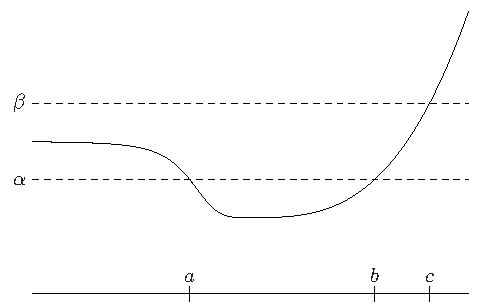
\includegraphics[width=.58\textwidth]{figures/ch03-110.pdf}
\caption*{图3.9 $\R$ 上的拟凸函数。对每个 $\alpha$，$\alpha$-下水平集 $S_\alpha$ 都凸，即为区间。下水平集 $S_\alpha$ 是 $[a,b]$，下水平集 $S_\beta$ 是 $(-\infty,c]$。}
\end{figure}
对于 $\R$ 上的函数，拟凸性要求每个下水平集都是区间，其中也可以包括无穷区间。图3.9给出了 $\R$ 上一个拟凸函数的例子。

凸函数的下水平集凸，因此凸函数都拟凸。但简单例子，例如图3.9，表明逆命题不成立。
\begin{origexample}{3.29}
$\R$ 上的几个例子：
\begin{itemize}
\item \textbf{对数。}$\R_{++}$ 上的 $\log x$ 拟凸，也拟凹，因而拟线性。
\item \textbf{向上取整函数。}$\operatorname{ceil}(x)=\inf\{z\in\Z\mid z\geq x\}$ 拟凸，也拟凹。
\end{itemize}
\end{origexample}
这些例子表明，拟凸函数可以是凹函数，也可以不连续。下面给出 $\R^n$ 上的一些例子。
\begin{origexample}{3.30}
\textbf{向量的长度。}将 $x\in\R^n$ 的长度定义为非零分量的最大下标，即
\[f(x)=\max\{i\mid x_i\ne0\}.\]
（规定零向量的长度为零。）此函数在 $\R^n$ 上拟凸，因为它的下水平集是子空间：
\[f(x)\leq\alpha\ \Longleftrightarrow\ x_i=0,\quad i=\lfloor\alpha\rfloor+1,\ldots,n.\]
\end{origexample}
\begin{origexample}{3.31}
考虑 $f:\R^2\to\R$，$\dom f=\R_+^2$，$f(x_1,x_2)=x_1x_2$。它既不凸也不凹，因为 Hessian
\[\nabla^2f(x)=\begin{bmatrix}0&1\\1&0\end{bmatrix}\]
% Source PDF page 111 (printed p. 97)
不定，有一个正特征值和一个负特征值。不过，$f$ 拟凹，因为对所有 $\alpha$，上水平集
\[\{x\in\R_+^2\mid x_1x_2\geq\alpha\}\]
都凸。（但 $f$ 在 $\R^2$ 上不拟凹。）
\end{origexample}
\begin{origexample}{3.32}
\textbf{线性分式函数。}函数
\[f(x)=\frac{a^\T x+b}{c^\T x+d},\qquad\dom f=\{x\mid c^\T x+d>0\},\]
既拟凸又拟凹，即拟线性。它的 $\alpha$-下水平集为
\[
\begin{aligned}
 S_\alpha&=\{x\mid c^\T x+d>0,\ (a^\T x+b)/(c^\T x+d)\leq\alpha\}\\
 &=\{x\mid c^\T x+d>0,\ a^\T x+b\leq\alpha(c^\T x+d)\},
\end{aligned}
\]
它凸，因为它是一个开半空间和一个闭半空间的交。（同样可以证明上水平集凸。）
\end{origexample}
\begin{origexample}{3.33}
\textbf{距离比函数。}设 $a,b\in\R^n$，定义
\[f(x)=\frac{\norm{x-a}_2}{\norm{x-b}_2},\]
即到 $a$ 的欧氏距离与到 $b$ 的欧氏距离之比。那么，$f$ 在半空间 $\{x\mid\norm{x-a}_2\leq\norm{x-b}_2\}$ 上拟凸。为证明这一点，考虑 $f$ 的 $\alpha$-下水平集，其中取 $\alpha\leq1$，因为在上述半空间上 $f(x)\leq1$。这个下水平集由满足
\[\norm{x-a}_2\leq\alpha\norm{x-b}_2\]
的点组成。两边平方并整理，可见它等价于
\[(1-\alpha^2)x^\T x-2(a-\alpha^2b)^\T x+a^\T a-\alpha^2b^\T b\leq0.\]
当 $\alpha\leq1$ 时，这描述了一个凸集，事实上是一个欧氏球。
\end{origexample}
\begin{origexample}{3.34}
\textbf{内部收益率。}用 $x=(x_0,x_1,\ldots,x_n)$ 表示跨越 $n$ 个时期的现金流序列，其中 $x_i>0$ 表示第 $i$ 期收到的款项，$x_i<0$ 表示第 $i$ 期支付的款项。利率为 $r\geq0$ 时，现金流的现值定义为
\[\operatorname{PV}(x,r)=\sum_{i=0}^n(1+r)^{-i}x_i.\]
（因子 $(1+r)^{-i}$ 是第 $i$ 期支付或收到款项的贴现因子。）

现在考虑满足 $x_0<0$、$x_0+x_1+\cdots+x_n>0$ 的现金流。这意味着在第零期先投资 $|x_0|$，其余现金流之和 $x_1+\cdots+x_n$，在不计贴现的情况下，超过初始投资。
% Source PDF page 112 (printed p. 98)
对于这样的现金流，$\operatorname{PV}(x,0)>0$，而 $r\to\infty$ 时 $\operatorname{PV}(x,r)\to x_0<0$，因此至少存在一个 $r\geq0$ 使 $\operatorname{PV}(x,r)=0$。将现金流的内部收益率定义为使现值为零的最小非负利率：
\[\operatorname{IRR}(x)=\inf\{r\geq0\mid\operatorname{PV}(x,r)=0\}.\]
内部收益率关于 $x$ 拟凹，这里限制 $x_0<0$、$x_1+\cdots+x_n>0$。注意到
\[\operatorname{IRR}(x)\geq R\ \Longleftrightarrow\
 \operatorname{PV}(x,r)>0\text{ 对 }0\leq r<R\text{ 成立}.\]
左端定义了 IRR 的 $R$-上水平集。右端是在 $0\leq r<R$ 范围内，以 $r$ 为指标的集合 $\{x\mid\operatorname{PV}(x,r)>0\}$ 的交。对每个 $r$，$\operatorname{PV}(x,r)>0$ 定义一个开半空间，因此右端为凸集。
\end{origexample}
\subsection{基本性质}
上述例子表明，拟凸性大大推广了凸性。尽管如此，凸函数的许多性质仍然适用于拟凸函数，或者有对应的形式。例如，有一个刻画拟凸性的 Jensen 不等式变体：函数 $f$ 拟凸，当且仅当 $\dom f$ 凸，并且对任意 $x,y\in\dom f$、$0\leq\theta\leq1$，有
\begin{equation}f(\theta x+(1-\theta)y)\leq\max\{f(x),f(y)\},\tag{3.19}\end{equation}
也就是说，线段上函数值不超过两端函数值的最大值。式(3.19)有时称为拟凸函数的 Jensen 不等式，图3.10说明了这一点。
\begin{origexample}{3.35}
\textbf{非负向量的基数。}向量 $x\in\R^n$ 的基数或大小是非零分量的个数，记为 $\operatorname{card}(x)$。函数 $\operatorname{card}$ 在 $\R_+^n$ 上拟凹，但在 $\R^n$ 上不拟凹。由对 $x,y\succeq0$ 成立的修正 Jensen 不等式
\[\operatorname{card}(x+y)\geq\min\{\operatorname{card}(x),\operatorname{card}(y)\}\]
可立即得出这一点。
\end{origexample}
\begin{origexample}{3.36}
\textbf{半正定矩阵的秩。}函数 $\rank X$ 在 $\mathbb S_+^n$ 上拟凹。这来自对 $X,Y\in\mathbb S_+^n$ 成立的修正 Jensen 不等式(3.19)：
\[\rank(X+Y)\geq\min\{\rank X,\rank Y\}.\]
它可以视为上一个例子的推广，因为对 $x\succeq0$ 有 $\rank(\diag(x))=\operatorname{card}(x)$。
\end{origexample}
% Source PDF page 113 (printed p. 99)
\begin{figure}[htbp]\centering
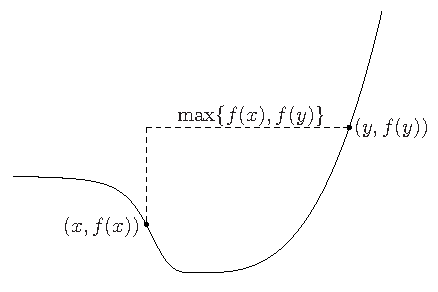
\includegraphics[width=.52\textwidth]{figures/ch03-113.pdf}
\caption*{图3.10 $\R$ 上的拟凸函数。在 $x$ 和 $y$ 之间，$f$ 的值不超过 $\max\{f(x),f(y)\}$。}
\end{figure}
如同凸性，拟凸性也由函数 $f$ 在直线上的表现刻画：$f$ 拟凸，当且仅当它在任意与定义域相交的直线上的限制拟凸。特别地，可以把函数限制在任意直线上，再检验所得 $\R$ 上函数的拟凸性，以验证原函数拟凸。
\subsubsection*{$\R$ 上的拟凸函数}
可以简单地刻画 $\R$ 上的拟凸函数。这里考虑连续函数，因为一般情况下条件的表述比较繁琐。连续函数 $f:\R\to\R$ 拟凸，当且仅当下列条件至少有一个成立：
\begin{itemize}
\item $f$ 单调不减；
\item $f$ 单调不增；
\item 存在 $c\in\dom f$，当 $t\leq c$ 且 $t\in\dom f$ 时，$f$ 单调不增；当 $t\geq c$ 且 $t\in\dom f$ 时，$f$ 单调不减。
\end{itemize}
点 $c$ 可选为 $f$ 的任意全局最小点，见图3.11。
\subsection{可微拟凸函数}
\subsubsection*{一阶条件}
设 $f:\R^n\to\R$ 可微。那么，$f$ 拟凸，当且仅当 $\dom f$ 凸，且对所有 $x,y\in\dom f$ 有
\begin{equation}f(y)\leq f(x)\ \Longrightarrow\ \nabla f(x)^\T(y-x)\leq0.\tag{3.20}\end{equation}
% Source PDF page 114 (printed p. 100)
\begin{figure}[htbp]\centering
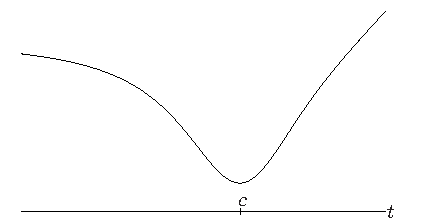
\includegraphics[width=.56\textwidth]{figures/ch03-114a.pdf}
\caption*{图3.11 $\R$ 上的拟凸函数。当 $t\leq c$ 时函数单调不增，当 $t\geq c$ 时单调不减。}
\end{figure}
\begin{figure}[htbp]\centering
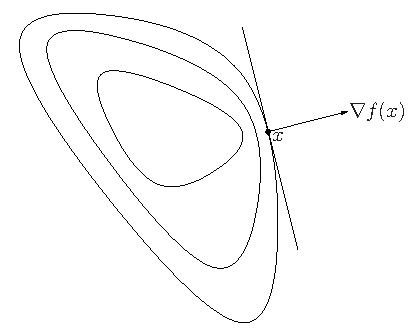
\includegraphics[width=.52\textwidth]{figures/ch03-114b.pdf}
\caption*{图3.12 拟凸函数 $f$ 的三条等高线。向量 $\nabla f(x)$ 确定了下水平集 $\{z\mid f(z)\leq f(x)\}$ 在 $x$ 处的一个支撑超平面。}
\end{figure}
这是不等式(3.2)对拟凸函数的对应形式。证明留作习题3.43。

当 $\nabla f(x)\ne0$ 时，条件(3.20)有一个简单的几何解释：$\nabla f(x)$ 确定下水平集 $\{y\mid f(y)\leq f(x)\}$ 在点 $x$ 处的支撑超平面，见图3.12。

虽然凸性的一阶条件(3.2)与拟凸性的一阶条件(3.20)相似，二者仍有重要差别。例如，若 $f$ 凸且 $\nabla f(x)=0$，则 $x$ 是 $f$ 的全局最小点。但对拟凸函数，这个命题不成立：可能有 $\nabla f(x)=0$，而 $x$ 不是 $f$ 的全局最小点。
% Source PDF page 115 (printed p. 101)
\subsubsection*{二阶条件}
现在设 $f$ 二次可微。若 $f$ 拟凸，则对所有 $x\in\dom f$ 和所有 $y\in\R^n$，有
\begin{equation}y^\T\nabla f(x)=0\ \Longrightarrow\ y^\T\nabla^2f(x)y\geq0.\tag{3.21}\end{equation}
对于 $\R$ 上的拟凸函数，这简化为
\[f'(x)=0\ \Longrightarrow\ f''(x)\geq0,\]
即斜率为零的任意一点，二阶导数非负。对 $\R^n$ 上的拟凸函数，条件(3.21)的解释稍复杂。与 $n=1$ 相同，只要 $\nabla f(x)=0$，就必须有 $\nabla^2f(x)\succeq0$。当 $\nabla f(x)\ne0$ 时，条件(3.21)意味着 $\nabla^2f(x)$ 在 $(n-1)$ 维子空间 $\nabla f(x)^\perp$ 上半正定。这说明 $\nabla^2f(x)$ 至多有一个负特征值。

作为一个部分逆命题，若 $f$ 对所有 $x\in\dom f$ 和所有 $y\in\R^n$、$y\ne0$ 都满足
\begin{equation}y^\T\nabla f(x)=0\ \Longrightarrow\ y^\T\nabla^2f(x)y>0,\tag{3.22}\end{equation}
则 $f$ 拟凸。这一条件相当于要求：在 $\nabla f(x)=0$ 的点，$\nabla^2f(x)$ 正定；在其他点，$\nabla^2f(x)$ 在 $(n-1)$ 维子空间 $\nabla f(x)^\perp$ 上正定。
\subsubsection*{拟凸性二阶条件的证明}
将函数限制在任意直线上后，只需考虑 $f:\R\to\R$。

先证明，若 $f:\R\to\R$ 在区间 $(a,b)$ 上拟凸，就必须满足式(3.21)，即若 $c\in(a,b)$、$f'(c)=0$，则 $f''(c)\geq0$。若 $f'(c)=0$、$f''(c)<0$，则对充分小的正数 $\epsilon$ 有 $f(c-\epsilon)<f(c)$、$f(c+\epsilon)<f(c)$。因此，对充分小的正数 $\epsilon$，下水平集 $\{x\mid f(x)\leq f(c)-\epsilon\}$ 不连通，从而不凸，与 $f$ 拟凸的假设矛盾。

再证明，若条件(3.22)成立，则 $f$ 拟凸。假设式(3.22)成立，即对每个满足 $f'(c)=0$ 的 $c\in(a,b)$，都有 $f''(c)>0$。这意味着，每当函数 $f'$ 穿过零值时，它严格增加，因此至多穿过零值一次。若 $f'$ 完全不穿过零值，则 $f$ 在 $(a,b)$ 上单调不增或单调不减，所以拟凸。否则，必恰好在某个 $c\in(a,b)$ 处穿过零。由于 $f''(c)>0$，有 $f'(t)\leq0$ 对 $a<t\leq c$ 成立，$f'(t)\geq0$ 对 $c\leq t<b$ 成立。这表明 $f$ 拟凸。
\subsection{保持拟凸性的运算}
\subsubsection*{非负加权最大值}
拟凸函数的非负加权最大值，即
\[f=\max\{w_1f_1,\ldots,w_mf_m\},\]
% Source PDF page 116 (printed p. 102)
其中 $w_i\geq0$、各 $f_i$ 拟凸，仍拟凸。这个性质可推广到一般的逐点上确界
\[f(x)=\sup_{y\in C}\bigl(w(y)g(x,y)\bigr),\]
其中 $w(y)\geq0$，且对每个 $y$，$g(x,y)$ 关于 $x$ 拟凸。这个事实容易验证：$f(x)\leq\alpha$ 当且仅当
\[w(y)g(x,y)\leq\alpha\qquad\text{对所有 }y\in C,\]
即 $f$ 的 $\alpha$-下水平集是各个关于变量 $x$ 的函数 $w(y)g(x,y)$ 的 $\alpha$-下水平集之交。
\begin{origexample}{3.37}
\textbf{广义特征值。}对称矩阵对 $(X,Y)$（$Y\succ0$）的最大广义特征值定义为
\[\lambda_{\max}(X,Y)=\sup_{u\ne0}\frac{u^\T Xu}{u^\T Yu}
 =\sup\{\lambda\mid\det(\lambda Y-X)=0\}.\]
见A.5.3节。此函数在 $\dom f=\mathbb S^n\times\mathbb S_{++}^n$ 上拟凸。

考虑表达式
\[\lambda_{\max}(X,Y)=\sup_{u\ne0}\frac{u^\T Xu}{u^\T Yu}.\]
对每个 $u\ne0$，$u^\T Xu/u^\T Yu$ 都是 $(X,Y)$ 的线性分式函数，从而关于 $(X,Y)$ 拟凸。因此，$\lambda_{\max}$ 作为一族拟凸函数的上确界，也拟凸。
\end{origexample}
\subsubsection*{复合}
若 $g:\R^n\to\R$ 拟凸、$h:\R\to\R$ 单调不减，则 $f=h\circ g$ 拟凸。

拟凸函数与仿射变换或线性分式变换复合，所得函数拟凸。若 $f$ 拟凸，则 $g(x)=f(Ax+b)$ 拟凸；$\widetilde g(x)=f((Ax+b)/(c^\T x+d))$ 在集合
\[\{x\mid c^\T x+d>0,\ (Ax+b)/(c^\T x+d)\in\dom f\}\]
上拟凸。
\subsubsection*{最小化}
若 $f(x,y)$ 关于 $x,y$ 联合拟凸，且 $C$ 为凸集，则函数
\[g(x)=\inf_{y\in C}f(x,y)\]
拟凸。

为证明这一点，只需证明任意 $\alpha\in\R$ 对应的 $\{x\mid g(x)\leq\alpha\}$ 凸。由 $g$ 的定义，$g(x)\leq\alpha$ 当且仅当对任意 $\epsilon>0$，都存在 $y\in C$ 使 $f(x,y)\leq\alpha+\epsilon$。
% Source PDF page 117 (printed p. 103)
设 $x_1,x_2$ 为 $g$ 的 $\alpha$-下水平集中的两点。对任意 $\epsilon>0$，存在 $y_1,y_2\in C$ 使
\[f(x_1,y_1)\leq\alpha+\epsilon,\qquad f(x_2,y_2)\leq\alpha+\epsilon.\]
因为 $f$ 关于 $x,y$ 拟凸，对 $0\leq\theta\leq1$ 还有
\[f(\theta x_1+(1-\theta)x_2,\theta y_1+(1-\theta)y_2)\leq\alpha+\epsilon.\]
因此 $g(\theta x_1+(1-\theta)x_2)\leq\alpha$，证明了 $\{x\mid g(x)\leq\alpha\}$ 凸。
\subsection{用一族凸函数表示}
后面将用到拟凸函数 $f$ 的下水平集的表示：这些集合凸，可以用凸函数的不等式描述。我们寻找一族以 $t\in\R$ 为指标的凸函数 $\phi_t:\R^n\to\R$，满足
\begin{equation}f(x)\leq t\ \Longleftrightarrow\ \phi_t(x)\leq0,\tag{3.23}\end{equation}
即拟凸函数 $f$ 的 $t$-下水平集是凸函数 $\phi_t$ 的零下水平集。显然，$\phi_t$ 必须满足：对所有 $x\in\R^n$，$\phi_t(x)\leq0$ 蕴含 $s\geq t$ 时 $\phi_s(x)\leq0$。若对每个 $x$，$\phi_t(x)$ 关于 $t$ 单调不增，即 $s\geq t$ 时 $\phi_s(x)\leq\phi_t(x)$，就满足这一性质。

为了说明这样的表示总存在，可取
\[\phi_t(x)=\begin{cases}0,&f(x)\leq t,\\\infty,&\text{其他情况},\end{cases}\]
即 $\phi_t$ 是 $f$ 的 $t$-下水平集的示性函数。显然表示不唯一；例如，若 $f$ 的下水平集闭，可取
\[\phi_t(x)=\dist\bigl(x,\{z\mid f(z)\leq t\}\bigr).\]
我们通常希望 $\phi_t$ 具有良好性质，例如可微性。
\begin{origexample}{3.38}
\textbf{凸函数除以凹函数。}设 $p$ 凸、$q$ 凹，并在凸集 $C$ 上满足 $p(x)\geq0$、$q(x)>0$。则定义在 $C$ 上的函数 $f(x)=p(x)/q(x)$ 拟凸。

因为
\[f(x)\leq t\ \Longleftrightarrow\ p(x)-tq(x)\leq0,\]
可以在 $t\geq0$ 时取 $\phi_t(x)=p(x)-tq(x)$。对每个 $t$，$\phi_t$ 凸；对每个 $x$，$\phi_t(x)$ 随 $t$ 递减。
\end{origexample}
% Source PDF page 118 (printed p. 104)
\section{对数凹函数与对数凸函数}
\subsection{定义}
若函数 $f:\R^n\to\R$ 对所有 $x\in\dom f$ 满足 $f(x)>0$，且 $\log f$ 凹，则称 $f$ 对数凹。若 $\log f$ 凸，则称它对数凸。因此，$f$ 对数凸，当且仅当 $1/f$ 对数凹。也可以方便地允许 $f$ 取零值，此时约定 $\log f(x)=-\infty$；在这种情况下，若扩展值函数 $\log f$ 凹，仍称 $f$ 对数凹。

对数凹性也可以不用对数而直接表达：定义域凸、且在定义域上恒正的函数 $f:\R^n\to\R$ 对数凹，当且仅当对所有 $x,y\in\dom f$、$0\leq\theta\leq1$，有
\[f(\theta x+(1-\theta)y)\geq f(x)^\theta f(y)^{1-\theta}.\]
特别地，对数凹函数在两点平均值处的函数值，至少为这两点函数值的几何平均。

由复合规则，若 $h$ 凸，则 $e^h$ 凸，因此对数凸函数是凸函数。类似地，非负凹函数对数凹。由于对数单调增加，对数凸函数显然拟凸，对数凹函数显然拟凹。
\begin{origexample}{3.39}
对数凹函数和对数凸函数的几个简单例子。
\begin{itemize}
\item \textbf{仿射函数。}$f(x)=a^\T x+b$ 在 $\{x\mid a^\T x+b>0\}$ 上对数凹。
\item \textbf{幂。}$\R_{++}$ 上的 $f(x)=x^a$，当 $a\leq0$ 时对数凸，当 $a\geq0$ 时对数凹。
\item \textbf{指数。}$f(x)=e^{ax}$ 既对数凸又对数凹。
\item 高斯密度的累积分布函数
\[\Phi(x)=\frac1{\sqrt{2\pi}}\int_{-\infty}^x e^{-u^2/2}\,du\]
对数凹（见习题3.54）。
\item \textbf{Gamma 函数。}Gamma 函数
\[\Gamma(x)=\int_0^\infty u^{x-1}e^{-u}\,du\]
在 $x\geq1$ 时对数凸（见习题3.52）。
\item \textbf{行列式。}$\det X$ 在 $\mathbb S_{++}^n$ 上对数凹。
\item \textbf{行列式除以迹。}$\det X/\tr X$ 在 $\mathbb S_{++}^n$ 上对数凹（见习题3.49）。
\end{itemize}
\end{origexample}
\begin{origexample}{3.40}
\textbf{对数凹密度函数。}许多常见的概率密度函数对数凹。两个例子是多元正态分布
\[f(x)=\frac1{\sqrt{(2\pi)^n\det\Sigma}}
 e^{-\frac12(x-\bar x)^\T\Sigma^{-1}(x-\bar x)}\]
% Source PDF page 119 (printed p. 105)
其中 $\bar x\in\R^n$、$\Sigma\in\mathbb S_{++}^n$，以及 $\R_+^n$ 上的指数分布
\[f(x)=\left(\prod_{i=1}^n\lambda_i\right)e^{-\lambda^\T x},\]
其中 $\lambda\succ0$。另一个例子是凸集 $C$ 上的均匀分布，
\[f(x)=\begin{cases}1/\alpha,&x\in C,\\0,&x\notin C,\end{cases}\]
其中 $\alpha=\vol(C)$ 是 $C$ 的体积，即 Lebesgue 测度。此时，$\log f$ 在 $C$ 外取 $-\infty$，在 $C$ 上取 $-\log\alpha$，因此凹。

再看一个较少见的例子，Wishart 分布。其定义如下：设 $x_1,\ldots,x_p\in\R^n$ 是独立高斯随机向量，均值为零、协方差为 $\Sigma\in\mathbb S^n$，其中 $p>n$。随机矩阵 $X=\sum_{i=1}^p x_ix_i^\T$ 的 Wishart 密度为
\[f(X)=a(\det X)^{(p-n-1)/2}e^{-\frac12\tr(\Sigma^{-1}X)},\]
$\dom f=\mathbb S_{++}^n$，$a$ 为正常数。Wishart 密度对数凹，因为
\[\log f(X)=\log a+\frac{p-n-1}2\log\det X-\frac12\tr(\Sigma^{-1}X)\]
是 $X$ 的凹函数。
\end{origexample}
\subsection{性质}
\subsubsection*{二次可微的对数凸函数与对数凹函数}
设 $f$ 二次可微，$\dom f$ 凸，则
\[\nabla^2\log f(x)=\frac1{f(x)}\nabla^2 f(x)
 -\frac1{f(x)^2}\nabla f(x)\nabla f(x)^\T.\]
因此，$f$ 对数凸，当且仅当对所有 $x\in\dom f$ 有
\[f(x)\nabla^2 f(x)\succeq\nabla f(x)\nabla f(x)^\T;\]
$f$ 对数凹，当且仅当对所有 $x\in\dom f$ 有
\[f(x)\nabla^2 f(x)\preceq\nabla f(x)\nabla f(x)^\T.\]
\subsubsection*{乘法、加法与积分}
对数凸性和对数凹性在乘法与正数乘法下封闭。例如，若 $f,g$ 对数凹，则逐点乘积 $h(x)=f(x)g(x)$ 也对数凹，因为 $\log h(x)=\log f(x)+\log g(x)$，且 $\log f(x)$、$\log g(x)$ 都是 $x$ 的凹函数。

简单例子表明，对数凹函数之和一般不对数凹。不过，加法保持对数凸性。设 $f,g$ 对数凸，即 $F=\log f$、$G=\log g$ 凸。由凸函数的复合规则，
\[\log(\exp F+\exp G)=\log(f+g)\]
% Source PDF page 120 (printed p. 106)
凸。因此，两个对数凸函数之和对数凸。

更一般地，若对每个 $y\in C$，$f(x,y)$ 关于 $x$ 对数凸，则
\[g(x)=\int_C f(x,y)\,dy\]
对数凸。
\begin{origexample}{3.41}
\textbf{非负函数的 Laplace 变换、矩母函数与累积量母函数。}设 $p:\R^n\to\R$ 对所有 $x$ 满足 $p(x)\geq0$。$p$ 的 Laplace 变换
\[P(z)=\int p(x)e^{-z^\T x}\,dx\]
在 $\R^n$ 上对数凸。（自然地，$\dom P=\{z\mid P(z)<\infty\}$。）

再设 $p$ 是密度，即 $\int p(x)\,dx=1$。函数 $M(z)=P(-z)$ 称为该密度的矩母函数。其名称来自：在 $z=0$ 处计算矩母函数的导数，即可得到密度的各阶矩。例如，
\[\nabla M(0)=\E v,\qquad\nabla^2M(0)=\E vv^\T,\]
其中 $v$ 是密度为 $p$ 的随机变量。

凸函数 $\log M(z)$ 称为 $p$ 的累积量母函数，因为它的导数给出密度的累积量。例如，累积量母函数在零处的一阶、二阶导数，分别为相关随机变量的均值和协方差：
\[\nabla\log M(0)=\E v,\qquad
 \nabla^2\log M(0)=\E(v-\E v)(v-\E v)^\T.\]
\end{origexample}
\subsubsection*{对数凹函数的积分}
在某些特殊情况下，积分保持对数凹性。若 $f:\R^n\times\R^m\to\R$ 对数凹，则
\[g(x)=\int f(x,y)\,dy\]
是 $x$ 的对数凹函数，定义在 $\R^n$ 上。这里积分在 $\R^m$ 上进行。这个结论的证明并不简单，见参考文献。

这个结论有许多重要推论，本节余下部分将介绍其中一些。例如，它说明对数凹概率密度的边缘分布仍对数凹，也说明对数凹性在卷积下封闭：若 $f,g$ 在 $\R^n$ 上对数凹，则卷积
\[(f*g)(x)=\int f(x-y)g(y)\,dy\]
也对数凹。因为 $g(y)$ 和 $f(x-y)$ 关于 $(x,y)$ 对数凹，所以乘积 $f(x-y)g(y)$ 也对数凹，再应用积分结论即可。
% Source PDF page 121 (printed p. 107)
设 $C\subseteq\R^n$ 是凸集，$w$ 为 $\R^n$ 中的随机向量，具有对数凹概率密度 $p$。则函数
\[f(x)=\Prob(x+w\in C)\]
关于 $x$ 对数凹。将 $f$ 表示为
\[f(x)=\int g(x+w)p(w)\,dw,\]
其中
\[g(u)=\begin{cases}1,&u\in C,\\0,&u\notin C,\end{cases}\]
对数凹，再应用积分结论即可。
\begin{origexample}{3.42}
概率密度函数 $f:\R^n\to\R$ 的累积分布函数定义为
\[F(x)=\Prob(w\preceq x)=\int_{-\infty}^{x_n}\cdots\int_{-\infty}^{x_1}
 f(z)\,dz_1\cdots dz_n,\]
其中 $w$ 是密度为 $f$ 的随机变量。若 $f$ 对数凹，则 $F$ 对数凹。前面已经遇到一个特例：高斯随机变量的累积分布函数
\[f(x)=\frac1{\sqrt{2\pi}}\int_{-\infty}^x e^{-t^2/2}\,dt\]
对数凹，见例3.39和习题3.54。
\end{origexample}
\begin{origexample}{3.43}
\textbf{成品率函数。}用 $x\in\R^n$ 表示生产某种产品时一组参数的标称值或目标值。制造过程的波动使产品生产出来后的参数成为 $x+w$，其中随机向量 $w\in\R^n$ 表示制造波动，通常假设均值为零。制造过程的成品率作为标称参数值的函数，为
\[Y(x)=\Prob(x+w\in S),\]
其中 $S\subseteq\R^n$ 是产品可接受参数值的集合，即产品规格。

若制造误差 $w$ 的密度对数凹，例如高斯密度，并且产品规格集合 $S$ 凸，则成品率函数 $Y$ 对数凹。这意味着 $\alpha$-成品率区域，即成品率超过 $\alpha$ 的标称参数集合，凸。例如，95\% 成品率区域
\[\{x\mid Y(x)\geq0.95\}=\{x\mid\log Y(x)\geq\log0.95\}\]
凸，因为它是凹函数 $\log Y$ 的上水平集。
\end{origexample}
% Source PDF page 122 (printed p. 108)
\begin{origexample}{3.44}
\textbf{多面体的体积。}设 $A\in\R^{m\times n}$，定义
\[P_u=\{x\in\R^n\mid Ax\preceq u\}.\]
则它的体积 $\vol P_u$ 是 $u$ 的对数凹函数。

注意函数
\[\Psi(x,u)=\begin{cases}1,&Ax\preceq u,\\0,&\text{其他情况},\end{cases}\]
对数凹。由积分结论，
\[\int\Psi(x,u)\,dx=\vol P_u\]
对数凹。
\end{origexample}
\section{相对于广义不等式的凸性}
现在用广义不等式代替 $\R$ 上的通常次序，推广单调性和凸性的概念。
\subsection{相对于广义不等式的单调性}
设 $K\subseteq\R^n$ 是正常锥，对应广义不等式 $\preceq_K$。若函数 $f:\R^n\to\R$ 满足
\[x\preceq_K y\ \Longrightarrow\ f(x)\leq f(y),\]
则称它为 $K$-单调不减函数；若满足
\[x\preceq_K y,\ x\ne y\ \Longrightarrow\ f(x)<f(y),\]
则称它为 $K$-严格递增函数。类似地定义 $K$-单调不增和 $K$-严格递减函数。
\begin{origexample}{3.45}
\textbf{向量的单调函数。}函数 $f:\R^n\to\R$ 相对于 $\R_+^n$ 单调不减，当且仅当对所有 $x,y$，有
\[x_1\leq y_1,\ldots,x_n\leq y_n\ \Longrightarrow\ f(x)\leq f(y).\]
这等同于：将 $f$ 限制在任一分量 $x_i$ 上，即把 $x_i$ 作为变量、固定 $j\ne i$ 的各 $x_j$ 时，所得函数单调不减。
\end{origexample}
\begin{origexample}{3.46}
\textbf{矩阵单调函数。}若函数 $f:\mathbb S^n\to\R$ 相对于半正定锥单调，则称它为矩阵单调函数，对应地有矩阵递增、矩阵递减。关于变量 $X\in\mathbb S^n$ 的几个矩阵单调函数例子如下：
% Source PDF page 123 (printed p. 109)
\begin{itemize}
\item $\tr(WX)$，其中 $W\in\mathbb S^n$。若 $W\succeq0$，它矩阵单调不减；若 $W\succ0$，它矩阵严格递增；若 $W\preceq0$，它矩阵单调不增；若 $W\prec0$，它矩阵严格递减。
\item $\tr(X^{-1})$ 在 $\mathbb S_{++}^n$ 上矩阵严格递减。
\item $\det X$ 在 $\mathbb S_{++}^n$ 上矩阵严格递增，在 $\mathbb S_+^n$ 上矩阵单调不减。
\end{itemize}
\end{origexample}
\subsubsection*{单调性的梯度条件}
回顾：具有凸定义域（即区间）的可微函数 $f:\R\to\R$ 单调不减，当且仅当对所有 $x\in\dom f$ 有 $f'(x)\geq0$；若所有点都有 $f'(x)>0$，则函数严格递增，但逆命题不成立。这些条件容易推广到相对于广义不等式的单调性。具有凸定义域的可微函数 $f$ 为 $K$-单调不减函数，当且仅当对所有 $x\in\dom f$ 有
\begin{equation}\nabla f(x)\succeq_{K^*}0.\tag{3.24}\end{equation}
与简单标量情形的区别是：梯度必须在对偶不等式意义下非负。严格情形有如下结论：若对所有 $x\in\dom f$ 有
\begin{equation}\nabla f(x)\succ_{K^*}0,\tag{3.25}\end{equation}
则 $f$ 为 $K$-严格递增函数。如同标量情形，逆命题不成立。

下面证明这些单调性一阶条件。先假设 $f$ 对所有 $x$ 满足式(3.24)，但不为 $K$-单调不减函数，即存在 $x,y$，$x\preceq_K y$ 且 $f(y)<f(x)$。由可微性，存在 $t\in[0,1]$ 使
\[\frac d{dt}f(x+t(y-x))=\nabla f(x+t(y-x))^\T(y-x)<0.\]
因为 $y-x\in K$，这意味着
\[\nabla f(x+t(y-x))\notin K^*,\]
与式(3.24)处处成立的假设矛盾。同样可以证明，式(3.25)蕴含 $f$ 为 $K$-严格递增函数。

式(3.24)处处成立的必要性也容易看出。假设式(3.24)在 $x=z$ 处不成立。由对偶锥定义，存在 $v\in K$ 使
\[\nabla f(z)^\T v<0.\]
考虑关于 $t$ 的函数 $h(t)=f(z+tv)$，有 $h'(0)=\nabla f(z)^\T v<0$，所以存在 $t>0$，使 $h(t)=f(z+tv)<h(0)=f(z)$，即 $f$ 不是 $K$-单调不减函数。
\subsection{相对于广义不等式的凸性}
设 $K\subseteq\R^m$ 为正常锥，对应广义不等式 $\preceq_K$。若对所有 $x,y$ 以及 $0\leq\theta\leq1$，有
\[f(\theta x+(1-\theta)y)\preceq_K\theta f(x)+(1-\theta)f(y),\]
则称 $f:\R^n\to\R^m$ 为 $K$-凸函数。
% Source PDF page 124 (printed p. 110)
若对所有 $x\ne y$、$0<\theta<1$，有
\[f(\theta x+(1-\theta)y)\prec_K\theta f(x)+(1-\theta)f(y),\]
则称为严格 $K$-凸函数。当 $m=1$、$K=\R_+$ 时，这些定义退化为通常的凸性和严格凸性。
\begin{origexample}{3.47}
\textbf{相对于逐分量不等式的凸性。}函数 $f:\R^n\to\R^m$ 相对于逐分量不等式（即 $\R_+^m$ 诱导的广义不等式）凸，当且仅当对所有 $x,y$、$0\leq\theta\leq1$ 有
\[f(\theta x+(1-\theta)y)\preceq\theta f(x)+(1-\theta)f(y),\]
即每个分量 $f_i$ 都是凸函数。函数 $f$ 相对于逐分量不等式严格凸，当且仅当每个分量 $f_i$ 严格凸。
\end{origexample}
\begin{origexample}{3.48}
\textbf{矩阵凸性。}设 $f$ 为对称矩阵值函数，即 $f:\R^n\to\mathbb S^m$。若对任意 $x,y$ 以及 $\theta\in[0,1]$，有
\[f(\theta x+(1-\theta)y)\preceq\theta f(x)+(1-\theta)f(y),\]
则称 $f$ 相对于矩阵不等式凸，有时称为矩阵凸性。等价的定义是：对所有向量 $z$，标量函数 $z^\T f(x)z$ 凸。这常是证明矩阵凸性的好方法。若当 $x\ne y$、$0<\theta<1$ 时有
\[f(\theta x+(1-\theta)y)\prec\theta f(x)+(1-\theta)f(y),\]
则称 $f$ 严格矩阵凸；等价地，对每个 $z\ne0$，$z^\T fz$ 都严格凸。几个例子如下：
\begin{itemize}
\item 函数 $f(X)=XX^\T$、$X\in\R^{n\times m}$ 矩阵凸，因为对固定 $z$，$z^\T XX^\T z=\norm{X^\T z}_2^2$ 是关于 $X$ 的各分量的凸二次函数。同样，$f(X)=X^2$ 在 $\mathbb S^n$ 上矩阵凸。
\item 当 $1\leq p\leq2$ 或 $-1\leq p\leq0$ 时，$X^p$ 在 $\mathbb S_{++}^n$ 上矩阵凸；当 $0\leq p\leq1$ 时，它矩阵凹。
\item 当 $n\geq2$ 时，函数 $f(X)=e^X$ 在 $\mathbb S^n$ 上不矩阵凸。
\end{itemize}
\end{origexample}
凸函数的许多结论可以推广到 $K$-凸函数。一个简单例子是：函数 $K$-凸，当且仅当它在定义域内任意直线上的限制 $K$-凸。本节余下部分列举几个后面会用到的 $K$-凸性结论；更多结论将在习题中讨论。
\subsubsection*{$K$-凸性的对偶刻画}
函数 $f$ 为 $K$-凸函数，当且仅当对每个 $w\succeq_{K^*}0$，实值函数 $w^\T f$ 在通常意义下凸。函数 $f$ 严格 $K$-凸，当且仅当对每个非零 $w\succeq_{K^*}0$，函数 $w^\T f$ 严格凸。这些结论直接来自对偶不等式的定义与性质。
% Source PDF page 125 (printed p. 111)
\subsubsection*{可微 $K$-凸函数}
可微函数 $f$ 为 $K$-凸函数，当且仅当其定义域凸，并对所有 $x,y\in\dom f$ 有
\[f(y)\succeq_K f(x)+Df(x)(y-x).\]
这里 $Df(x)\in\R^{m\times n}$ 是 $f$ 在 $x$ 处的导数或 Jacobian 矩阵，见A.4.1节。

函数 $f$ 严格 $K$-凸，当且仅当对所有 $x,y\in\dom f$、$x\ne y$，有
\[f(y)\succ_K f(x)+Df(x)(y-x).\]
\subsubsection*{复合定理}
许多复合结论可以推广到 $K$-凸性。例如，若 $g:\R^n\to\R^p$ 为 $K$-凸函数，$h:\R^p\to\R$ 凸，且 $\widetilde h$（$h$ 的扩展值延拓）为 $K$-单调不减函数，则 $h\circ g$ 凸。这推广了“凸函数与单调不减的凸函数复合后仍凸”的结论。$\widetilde h$ 为 $K$-单调不减函数蕴含 $\dom h-K=\dom h$。
\begin{origexample}{3.49}
二次矩阵函数 $g:\R^{m\times n}\to\mathbb S^n$，
\[g(X)=X^\T AX+B^\T X+X^\T B+C,\]
其中 $A\in\mathbb S^m$、$B\in\R^{m\times n}$、$C\in\mathbb S^n$，当 $A\succeq0$ 时凸。

函数 $h:\mathbb S^n\to\R$，$h(Y)=-\log\det(-Y)$，在 $\dom h=-\mathbb S_{++}^n$ 上凸且递增。

由复合定理可知，
\[f(X)=-\log\det\bigl(-(X^\T AX+B^\T X+X^\T B+C)\bigr)\]
在
\[\dom f=\{X\in\R^{m\times n}\mid X^\T AX+B^\T X+X^\T B+C\prec0\}\]
上凸。这推广了如下事实：当 $a\geq0$ 时，
\[-\log(-(ax^2+bx+c))\]
在 $\{x\in\R\mid ax^2+bx+c<0\}$ 上凸。
\end{origexample}
% Source PDF page 126 (printed p. 112)
\section*{文献说明}
\addcontentsline{toc}{section}{文献说明}
凸分析的标准参考书是 Rockafellar [Roc70]。讨论凸函数的其他书籍包括 Stoer 和 Witzgall [SW70]、Roberts 和 Varberg [RV73]、Van Tiel [vT84]、Hiriart-Urruty 和 Lemaréchal [HUL93]、Ekeland 和 Témam [ET99]、Borwein 和 Lewis [BL00]、Florenzano 和 Le Van [FL01]、Barvinok [Bar02]，以及 Bertsekas、Nedić 和 Ozdaglar [Ber03]。多数非线性规划教材也有凸函数章节，例如 Mangasarian [Man94]、Bazaraa、Sherali 和 Shetty [BSS93]、Bertsekas [Ber99]、Polyak [Pol87]，以及 Peressini、Sullivan 和 Uhl [PSU88]。

Jensen 不等式见 [Jen06]。Hardy、Littlewood 和 Pólya [HLP52] 以及 Beckenbach 和 Bellman [BB65] 对不等式理论作了系统讨论，其中 Jensen 不等式起核心作用。

“透视函数”一词来自 Hiriart-Urruty 和 Lemaréchal [HUL93，第1卷，第100页]。例3.19中相对熵和 Kullback--Leibler 散度的定义，以及相关习题3.13，参见 Cover 和 Thomas [CT91]。

拟凸函数以及其他凸性推广的重要早期文献，包括 Nikaidô [Nik54]、Mangasarian [Man94，第9章]、Arrow 和 Enthoven [AE61]、Ponstein [Pon67]，以及 Luenberger [Lue68]。更全面的参考文献列表见 Bazaraa、Sherali 和 Shetty [BSS93，第126页]。

Prékopa [Pré80] 综述了对数凹函数。Barndorff-Nielsen [BN78，第7节] 提到 Laplace 变换的对数凸性。对数凹函数积分结论的证明，见 Prékopa [Pré71, Pré73]。

从 Nesterov 和 Nemirovski [NN94，第156页] 开始，广义不等式广泛用于近年来的锥规划文献；也见 Ben-Tal 和 Nemirovski [BTN01] 及第4章末尾的参考文献。相对于广义不等式的凸性也见于 Luenberger [Lue69，第8.2节] 和 Isii [Isi64] 的工作。矩阵单调性与矩阵凸性归于 Löwner [Löw34]；Davis [Dav63]、Roberts 和 Varberg [RV73，第216页]，以及 Marshall 和 Olkin [MO79，第16E节] 有详细讨论。例3.48中关于 $X^p$ 的凸性与凹性的结论，见 Bondar [Bon94，定理16.1]。一个说明 $e^X$ 不矩阵凸的简单例子，见 Marshall 和 Olkin [MO79，第474页]。
% Source PDF page 127 (printed p. 113)
\section*{习题}
\addcontentsline{toc}{section}{习题}
\subsection*{凸性的定义}
\paragraph{3.1}设 $f:\R\to\R$ 凸，$a,b\in\dom f$ 且 $a<b$。
\begin{enumerate}[label=(\alph*)]
\item 证明，对所有 $x\in[a,b]$，有
\[f(x)\leq\frac{b-x}{b-a}f(a)+\frac{x-a}{b-a}f(b).\]
\item 证明，对所有 $x\in(a,b)$，有
\[\frac{f(x)-f(a)}{x-a}\leq\frac{f(b)-f(a)}{b-a}\leq\frac{f(b)-f(x)}{b-x}.\]
画出说明这一不等式的示意图。
\item 设 $f$ 可微。利用(b)证明
\[f'(a)\leq\frac{f(b)-f(a)}{b-a}\leq f'(b).\]
这些不等式也可由式(3.2)得到：
\[f(b)\geq f(a)+f'(a)(b-a),\qquad f(a)\geq f(b)+f'(b)(a-b).\]
\item 设 $f$ 二次可微。利用(c)证明 $f''(a)\geq0$、$f''(b)\geq0$。
\end{enumerate}
\paragraph{3.2}\textit{凸函数、凹函数、拟凸函数与拟凹函数的水平集。}下图给出函数 $f$ 的几个水平集。标为1的曲线表示 $\{x\mid f(x)=1\}$，其他类似。
\begin{center}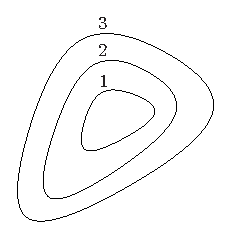
\includegraphics[width=.28\textwidth]{figures/ch03-ex127a.pdf}\end{center}
$f$ 是否可能凸、凹、拟凸或拟凹？说明理由。对下面的等高线重复上述问题。
\begin{center}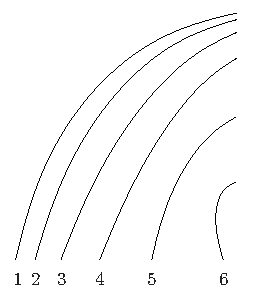
\includegraphics[width=.28\textwidth]{figures/ch03-ex127b.pdf}\end{center}
% Source PDF page 128 (printed p. 114)
\paragraph{3.3}\textit{递增凸函数的反函数。}设 $f:\R\to\R$ 在定义域 $(a,b)$ 上递增且凸。用 $g$ 表示它的反函数，即定义域为 $(f(a),f(b))$ 且对 $a<x<b$ 满足 $g(f(x))=x$ 的函数。关于 $g$ 的凸性或凹性，可以得到什么结论？
\paragraph{3.4}[RV73，第15页] 证明，连续函数 $f:\R^n\to\R$ 凸，当且仅当它在每条线段上的平均值不超过两个端点函数值的平均值：对任意 $x,y\in\R^n$，
\[\int_0^1 f(x+\lambda(y-x))\,d\lambda\leq\frac{f(x)+f(y)}2.\]
\paragraph{3.5}[RV73，第22页] \textit{凸函数的累积平均。}设 $f:\R\to\R$ 凸，$\R_+\subseteq\dom f$。证明，它的累积平均
\[F(x)=\frac1x\int_0^x f(t)\,dt,\qquad\dom F=\R_{++}\]
凸。\textit{提示：}对每个 $s$，$f(sx)$ 关于 $x$ 凸，因此 $\int_0^1 f(sx)\,ds$ 凸。
\paragraph{3.6}\textit{函数与上图。}函数的上图何时为半空间？何时为凸锥？何时为多面体？
\paragraph{3.7}设 $f:\R^n\to\R$ 凸，$\dom f=\R^n$，且在 $\R^n$ 上有上界。证明 $f$ 为常数。
\paragraph{3.8}\textit{凸性的二阶条件。}证明，二次可微函数 $f$ 凸，当且仅当其定义域凸，且对所有 $x\in\dom f$ 有 $\nabla^2f(x)\succeq0$。\textit{提示：}先考虑 $f:\R\to\R$。可以使用凸性的一阶条件，其证明见原书第70页。
\paragraph{3.9}\textit{仿射集上凸性的二阶条件。}设 $F\in\R^{n\times m}$、$\widehat x\in\R^n$。$f:\R^n\to\R$ 在仿射集 $\{Fz+\widehat x\mid z\in\R^m\}$ 上的限制定义为 $\widetilde f:\R^m\to\R$，其中
\[\widetilde f(z)=f(Fz+\widehat x),\qquad\dom\widetilde f=\{z\mid Fz+\widehat x\in\dom f\}.\]
设 $f$ 二次可微，且定义域凸。
\begin{enumerate}[label=(\alph*)]
\item 证明，$\widetilde f$ 凸，当且仅当对所有 $z\in\dom\widetilde f$ 有
\[F^\T\nabla^2f(Fz+\widehat x)F\succeq0.\]
\item 设 $A\in\R^{p\times n}$ 的零空间等于 $F$ 的值域，即 $AF=0$ 且 $\rank A=n-\rank F$。证明，若对所有 $z\in\dom\widetilde f$，存在 $\lambda\in\R$ 使
\[\nabla^2f(Fz+\widehat x)+\lambda A^\T A\succeq0,\]
则 $\widetilde f$ 凸。

\textit{提示：}使用如下结论：若 $B\in\mathbb S^n$、$A\in\R^{p\times n}$，并存在 $\lambda$ 使 $B+\lambda A^\T A\succeq0$，则对所有 $x\in\mathcal N(A)$ 有 $x^\T Bx\geq0$。
\end{enumerate}
\paragraph{3.10}\textit{Jensen 不等式的推广。}Jensen 不等式的一种解释是随机化或抖动会带来损失，即提高凸函数值的平均值：若 $f$ 凸、$v$ 为零均值随机变量，则 $\E f(x_0+v)\geq f(x_0)$。这引出如下猜想：若 $f$ 凸，则 $v$ 的方差越大，$\E f(x_0+v)$ 越大。
\begin{enumerate}[label=(\alph*)]
\item 给出反例说明这一猜想不成立。找出零均值随机变量 $v,w$，满足 $\operatorname{var}(v)>\operatorname{var}(w)$，以及凸函数 $f$ 和点 $x_0$，使 $\E f(x_0+v)<\E f(x_0+w)$。
% Source PDF page 129 (printed p. 115)
\item 当 $v,w$ 互为缩放时，这个猜想成立。证明，若 $f$ 凸且 $v$ 零均值，则 $\E f(x_0+tv)$ 在 $t\geq0$ 上单调增加。
\end{enumerate}
\paragraph{3.11}\textit{单调映射。}若函数 $\psi:\R^n\to\R^n$ 对所有 $x,y\in\dom\psi$ 满足
\[(\psi(x)-\psi(y))^\T(x-y)\geq0,\]
则称它单调。（这里“单调”的定义不同于3.6.1节，两种定义都广泛使用。）设 $f:\R^n\to\R$ 为可微凸函数。证明其梯度 $\nabla f$ 单调。逆命题是否成立，即每个单调映射都是某个凸函数的梯度吗？
\paragraph{3.12}设 $f:\R^n\to\R$ 凸、$g:\R^n\to\R$ 凹，$\dom f=\dom g=\R^n$，且对所有 $x$ 有 $g(x)\leq f(x)$。证明，存在仿射函数 $h$，对所有 $x$ 有 $g(x)\leq h(x)\leq f(x)$。换句话说，若凹函数 $g$ 是凸函数 $f$ 的下估计，则能在两者之间放入一个仿射函数。
\paragraph{3.13}\textit{Kullback--Leibler 散度与信息不等式。}设 $D_{\mathrm{kl}}$ 为式(3.17)定义的 Kullback--Leibler 散度。证明信息不等式：对所有 $u,v\in\R_{++}^n$ 有 $D_{\mathrm{kl}}(u,v)\geq0$。并证明 $D_{\mathrm{kl}}(u,v)=0$ 当且仅当 $u=v$。

\textit{提示：}Kullback--Leibler 散度可以表示为
\[D_{\mathrm{kl}}(u,v)=f(u)-f(v)-\nabla f(v)^\T(u-v),\]
其中 $f(v)=\sum_{i=1}^n v_i\log v_i$ 为 $v$ 的负熵。
\paragraph{3.14}\textit{凸—凹函数与鞍点。}若对每个固定的 $x$，$f(x,z)$ 关于 $z$ 凹，且对每个固定的 $z$，$f(x,z)$ 关于 $x$ 凸，则称 $f:\R^n\times\R^m\to\R$ 为凸—凹函数。还要求其定义域具有乘积形式 $\dom f=A\times B$，其中 $A\subseteq\R^n$、$B\subseteq\R^m$ 均凸。
\begin{enumerate}[label=(\alph*)]
\item 用 Hessian $\nabla^2f(x,z)$ 给出二次可微函数 $f:\R^n\times\R^m\to\R$ 为凸—凹函数的二阶条件。
\item 设 $f:\R^n\times\R^m\to\R$ 凸—凹且可微，$\nabla f(\widetilde x,\widetilde z)=0$。证明鞍点性质：对所有 $x,z$ 有
\[f(\widetilde x,z)\leq f(\widetilde x,\widetilde z)\leq f(x,\widetilde z).\]
证明这蕴含 $f$ 满足强极大极小性质：
\[\sup_z\inf_x f(x,z)=\inf_x\sup_z f(x,z),\]
两者的共同值为 $f(\widetilde x,\widetilde z)$。
\item 现在设 $f:\R^n\times\R^m\to\R$ 可微，但不必凸—凹，并在 $\widetilde x,\widetilde z$ 处具有鞍点性质：
\[f(\widetilde x,z)\leq f(\widetilde x,\widetilde z)\leq f(x,\widetilde z)\qquad\text{对所有 }x,z.\]
证明 $\nabla f(\widetilde x,\widetilde z)=0$。
\end{enumerate}
\subsection*{例子}
\paragraph{3.15}\textit{一族凹效用函数。}对 $0<\alpha\leq1$，令
\[u_\alpha(x)=\frac{x^\alpha-1}{\alpha},\qquad\dom u_\alpha=\R_+.\]
另定义 $u_0(x)=\log x$，$\dom u_0=\R_{++}$。
\begin{enumerate}[label=(\alph*)]
\item 证明，对 $x>0$，$u_0(x)=\lim_{\alpha\to0}u_\alpha(x)$。
% Source PDF page 130 (printed p. 116)
\item 证明各 $u_\alpha$ 凹、单调增加，并且都满足 $u_\alpha(1)=0$。
\end{enumerate}
这些函数常用于经济学，描述某种数量的商品或金钱所带来的收益或效用。$u_\alpha$ 的凹性意味着边际效用，即商品增加固定数量所获得的效用增量，随商品数量增加而减少。换句话说，凹性描述了饱和效应。
\paragraph{3.16}判断下列各函数是否凸、凹、拟凸或拟凹。
\begin{enumerate}[label=(\alph*)]
\item $\R$ 上的 $f(x)=e^x-1$。
\item $\R_{++}^2$ 上的 $f(x_1,x_2)=x_1x_2$。
\item $\R_{++}^2$ 上的 $f(x_1,x_2)=1/(x_1x_2)$。
\item $\R_{++}^2$ 上的 $f(x_1,x_2)=x_1/x_2$。
\item $\R\times\R_{++}$ 上的 $f(x_1,x_2)=x_1^2/x_2$。
\item $\R_{++}^2$ 上的 $f(x_1,x_2)=x_1^\alpha x_2^{1-\alpha}$，其中 $0\leq\alpha\leq1$。
\end{enumerate}
\paragraph{3.17}设 $p<1$、$p\ne0$。证明，函数
\[f(x)=\left(\sum_{i=1}^n x_i^p\right)^{1/p},\qquad\dom f=\R_{++}^n\]
凹。这包括特例 $f(x)=(\sum_{i=1}^n x_i^{1/2})^2$ 以及调和平均 $f(x)=(\sum_{i=1}^n1/x_i)^{-1}$。
\textit{提示：}改写3.1.5节中指数和对数函数及几何平均的证明。
\paragraph{3.18}改写3.1.5节中行列式对数函数凹性的证明，得到以下结论。
\begin{enumerate}[label=(\alph*)]
\item $f(X)=\tr(X^{-1})$ 在 $\dom f=\mathbb S_{++}^n$ 上凸。
\item $f(X)=(\det X)^{1/n}$ 在 $\dom f=\mathbb S_{++}^n$ 上凹。
\end{enumerate}
\paragraph{3.19}\textit{非负加权和与积分。}
\begin{enumerate}[label=(\alph*)]
\item 证明，$f(x)=\sum_{i=1}^r\alpha_i x_{[i]}$ 是 $x$ 的凸函数，其中 $\alpha_1\geq\alpha_2\geq\cdots\geq\alpha_r\geq0$，$x_{[i]}$ 是 $x$ 的第 $i$ 大分量。可以使用 $f(x)=\sum_{i=1}^k x_{[i]}$ 在 $\R^n$ 上凸这一事实。
\item 设 $T(x,\omega)$ 为三角多项式
\[T(x,\omega)=x_1+x_2\cos\omega+x_3\cos2\omega+\cdots+x_n\cos(n-1)\omega.\]
证明函数
\[f(x)=-\int_0^{2\pi}\log T(x,\omega)\,d\omega\]
在 $\{x\in\R^n\mid T(x,\omega)>0,\ 0\leq\omega\leq2\pi\}$ 上凸。
\end{enumerate}
\paragraph{3.20}\textit{与仿射函数复合。}证明以下函数 $f:\R^n\to\R$ 凸。
\begin{enumerate}[label=(\alph*)]
\item $f(x)=\norm{Ax-b}$，其中 $A\in\R^{m\times n}$、$b\in\R^m$，$\norm{\cdot}$ 为 $\R^m$ 上的范数。
\item $f(x)=-(\det(A_0+x_1A_1+\cdots+x_nA_n))^{1/m}$，定义域为 $\{x\mid A_0+x_1A_1+\cdots+x_nA_n\succ0\}$，其中 $A_i\in\mathbb S^m$。
\item $f(X)=\tr(A_0+x_1A_1+\cdots+x_nA_n)^{-1}$，定义域为 $\{x\mid A_0+x_1A_1+\cdots+x_nA_n\succ0\}$，其中 $A_i\in\mathbb S^m$。使用 $\tr(X^{-1})$ 在 $\mathbb S_{++}^m$ 上凸的结论，见习题3.18。
\end{enumerate}
% Source PDF page 131 (printed p. 117)
\paragraph{3.21}\textit{逐点最大值与上确界。}证明下列函数 $f:\R^n\to\R$ 凸。
\begin{enumerate}[label=(\alph*)]
\item $f(x)=\max_{i=1,\ldots,k}\norm{A^{(i)}x-b^{(i)}}$，其中 $A^{(i)}\in\R^{m\times n}$、$b^{(i)}\in\R^m$，$\norm{\cdot}$ 为 $\R^m$ 上的范数。
\item $f(x)=\sum_{i=1}^r|x|_{[i]}$，定义在 $\R^n$ 上，其中 $|x|$ 为满足 $|x|_i=|x_i|$ 的向量，即对 $x$ 逐分量取绝对值，$|x|_{[i]}$ 为 $|x|$ 的第 $i$ 大分量。换句话说，$|x|_{[1]},|x|_{[2]},\ldots,|x|_{[n]}$ 是 $x$ 的各分量绝对值按非增顺序排列后的结果。
\end{enumerate}
\paragraph{3.22}\textit{复合规则。}证明以下函数凸。
\begin{enumerate}[label=(\alph*)]
\item $f(x)=-\log(-\log(\sum_{i=1}^m e^{a_i^\T x+b_i}))$，$\dom f=\{x\mid\sum_{i=1}^m e^{a_i^\T x+b_i}<1\}$。可以使用 $\log(\sum_{i=1}^n e^{y_i})$ 凸的结论。
\item $f(x,u,v)=-\sqrt{uv-x^\T x}$，$\dom f=\{(x,u,v)\mid uv>x^\T x,\ u,v>0\}$。使用 $x^\T x/u$ 在 $u>0$ 时关于 $(x,u)$ 凸，以及 $-\sqrt{x_1x_2}$ 在 $\R_{++}^2$ 上凸这两个结论。
\item $f(x,u,v)=-\log(uv-x^\T x)$，$\dom f=\{(x,u,v)\mid uv>x^\T x,\ u,v>0\}$。
\item $f(x,t)=-(t^p-\norm x_p^p)^{1/p}$，其中 $p>1$，$\dom f=\{(x,t)\mid t\geq\norm x_p\}$。可以使用 $\norm x_p^p/u^{p-1}$ 在 $u>0$ 时关于 $(x,u)$ 凸（见习题3.23），以及 $-x^{1/p}y^{1-1/p}$ 在 $\R_+^2$ 上凸（见习题3.16）的结论。
\item $f(x,t)=-\log(t^p-\norm x_p^p)$，其中 $p>1$，$\dom f=\{(x,t)\mid t>\norm x_p\}$。可以使用 $\norm x_p^p/u^{p-1}$ 在 $u>0$ 时关于 $(x,u)$ 凸的结论，见习题3.23。
\end{enumerate}
\paragraph{3.23}\textit{函数的透视。}
\begin{enumerate}[label=(\alph*)]
\item 证明，当 $p>1$ 时，
\[f(x,t)=\frac{|x_1|^p+\cdots+|x_n|^p}{t^{p-1}}=\frac{\norm x_p^p}{t^{p-1}}\]
在 $\{(x,t)\mid t>0\}$ 上凸。
\item 证明
\[f(x)=\frac{\norm{Ax+b}_2^2}{c^\T x+d}\]
在 $\{x\mid c^\T x+d>0\}$ 上凸，其中 $A\in\R^{m\times n}$、$b\in\R^m$、$c\in\R^n$、$d\in\R$。
\end{enumerate}
\paragraph{3.24}\textit{概率单纯形上的一些函数。}设实值随机变量 $x$ 取值于 $\{a_1,\ldots,a_n\}$，其中 $a_1<a_2<\cdots<a_n$，且 $\Prob(x=a_i)=p_i$，$i=1,\ldots,n$。对下列各个关于 $p$ 的函数，在概率单纯形 $\{p\in\R_+^n\mid\one^\T p=1\}$ 上判断它是否凸、凹、拟凸或拟凹。
\begin{enumerate}[label=(\alph*)]
\item $\E x$。
\item $\Prob(x\geq\alpha)$。
\item $\Prob(\alpha\leq x\leq\beta)$。
\item $\sum_{i=1}^n p_i\log p_i$，即分布的负熵。
\item $\operatorname{var}x=\E(x-\E x)^2$。
\item $\operatorname{quartile}(x)=\inf\{\beta\mid\Prob(x\leq\beta)\geq0.25\}$。
\item 概率至少为90\% 的最小集合 $A\subseteq\{a_1,\ldots,a_n\}$ 的基数。基数指 $A$ 中元素的个数。
\item 包含90\% 概率的最窄区间的宽度，即
\[\inf\{\beta-\alpha\mid\Prob(\alpha\leq x\leq\beta)\geq0.9\}.\]
\end{enumerate}
% Source PDF page 132 (printed p. 118)
\paragraph{3.25}\textit{分布之间的最大概率距离。}设 $p,q\in\R^n$ 表示 $\{1,\ldots,n\}$ 上的两个概率分布，即 $p,q\succeq0$、$\one^\T p=\one^\T q=1$。将它们之间的最大概率距离 $d_{\mathrm{mp}}(p,q)$ 定义为所有事件上 $p,q$ 所赋概率之差的绝对值的最大值：
\[d_{\mathrm{mp}}(p,q)=\max\{|\Prob(p,C)-\Prob(q,C)|\mid C\subseteq\{1,\ldots,n\}\}.\]
这里 $\Prob(p,C)$ 为分布 $p$ 下 $C$ 的概率，即 $\Prob(p,C)=\sum_{i\in C}p_i$。

求出 $d_{\mathrm{mp}}$ 的一个简单表达式，用 $\norm{p-q}_1=\sum_{i=1}^n|p_i-q_i|$ 表示，并证明 $d_{\mathrm{mp}}$ 是 $\R^n\times\R^n$ 上的凸函数。它的定义域为 $\{(p,q)\mid p,q\succeq0,\ \one^\T p=\one^\T q=1\}$，但可以自然地延拓到整个 $\R^n\times\R^n$。
\paragraph{3.26}\textit{更多特征值函数。}设 $\lambda_1(X)\geq\lambda_2(X)\geq\cdots\geq\lambda_n(X)$ 为矩阵 $X\in\mathbb S^n$ 的特征值。前面已经看到几个关于 $X$ 凸或凹的特征值函数。
\begin{itemize}
\item 最大特征值 $\lambda_1(X)$ 凸（例3.10）；最小特征值 $\lambda_n(X)$ 凹。
\item 特征值之和，即迹 $\tr X=\lambda_1(X)+\cdots+\lambda_n(X)$，线性。
\item 特征值倒数之和，即逆矩阵的迹 $\tr(X^{-1})=\sum_{i=1}^n1/\lambda_i(X)$，在 $\mathbb S_{++}^n$ 上凸（习题3.18）。
\item 特征值的几何平均 $(\det X)^{1/n}=(\prod_{i=1}^n\lambda_i(X))^{1/n}$，以及特征值乘积的对数 $\log\det X=\sum_{i=1}^n\log\lambda_i(X)$，在 $X\in\mathbb S_{++}^n$ 上凹（习题3.18及原书第74页）。
\end{itemize}
本题利用变分刻画研究更多的特征值函数。
\begin{enumerate}[label=(\alph*)]
\item \textit{最大的 $k$ 个特征值之和。}证明 $\sum_{i=1}^k\lambda_i(X)$ 在 $\mathbb S^n$ 上凸。
\textit{提示：}[HJ85，第191页] 使用变分刻画
\[\sum_{i=1}^k\lambda_i(X)=\sup\{\tr(V^\T XV)\mid V\in\R^{n\times k},\ V^\T V=I\}.\]
\item \textit{最小的 $k$ 个特征值的几何平均。}证明 $(\prod_{i=n-k+1}^n\lambda_i(X))^{1/k}$ 在 $\mathbb S_{++}^n$ 上凹。
\textit{提示：}[MO79，第513页] 对 $X\succ0$，
\[\left(\prod_{i=n-k+1}^n\lambda_i(X)\right)^{1/k}
 =\frac1k\inf\{\tr(V^\T XV)\mid V\in\R^{n\times k},\ \det V^\T V=1\}.\]
\item \textit{最小的 $k$ 个特征值乘积的对数。}证明 $\sum_{i=n-k+1}^n\log\lambda_i(X)$ 在 $\mathbb S_{++}^n$ 上凹。
\textit{提示：}[MO79，第513页] 对 $X\succ0$，
\[\prod_{i=n-k+1}^n\lambda_i(X)
 =\inf\left\{\prod_{i=1}^k(V^\T XV)_{ii}\ \middle|\ V\in\R^{n\times k},\ V^\T V=I\right\}.\]
\end{enumerate}
\paragraph{3.27}\textit{Cholesky 因子的对角元。}每个 $X\in\mathbb S_{++}^n$ 都有唯一 Cholesky 分解 $X=LL^\T$，其中 $L$ 为下三角矩阵且 $L_{ii}>0$。证明 $L_{ii}$ 是 $X$ 的凹函数，定义域为 $\mathbb S_{++}^n$。

\textit{提示：}$L_{ii}$ 可表示为 $L_{ii}=(w-z^\T Y^{-1}z)^{1/2}$，其中
\[\begin{bmatrix}Y&z\\z^\T&w\end{bmatrix}\]
是 $X$ 的前 $i\times i$ 主子矩阵。
% Source PDF page 133 (printed p. 119)
\subsection*{保持凸性的运算}
\paragraph{3.28}\textit{把凸函数表示成一族仿射函数的逐点上确界。}本题将原书第83页证明的结论推广到 $\dom f\ne\R^n$。设 $f:\R^n\to\R$ 凸。定义 $\widetilde f:\R^n\to\R$ 为 $f$ 的所有仿射全局下估计的逐点上确界：
\[\widetilde f(x)=\sup\{g(x)\mid g\text{ 仿射},\ g(z)\leq f(z)\text{ 对所有 }z\text{ 成立}\}.\]
\begin{enumerate}[label=(\alph*)]
\item 证明，对 $x\in\operatorname{int}\dom f$，$f(x)=\widetilde f(x)$。
\item 证明，若 $f$ 闭，即 $\epi f$ 为闭集（见A.3.3节），则 $f=\widetilde f$。
\end{enumerate}
\paragraph{3.29}\textit{分段线性凸函数的表示。}凸函数 $f:\R^n\to\R$、$\dom f=\R^n$，若存在 $\R^n$ 的划分
\[\R^n=X_1\cup X_2\cup\cdots\cup X_L,\]
其中 $\operatorname{int}X_i\ne\varnothing$，且 $i\ne j$ 时 $\operatorname{int}X_i\cap\operatorname{int}X_j=\varnothing$，并有一族仿射函数 $a_1^\T x+b_1,\ldots,a_L^\T x+b_L$，使得 $x\in X_i$ 时 $f(x)=a_i^\T x+b_i$，则称 $f$ 分段线性。

证明，此类函数具有形式 $f(x)=\max\{a_1^\T x+b_1,\ldots,a_L^\T x+b_L\}$。
\paragraph{3.30}\textit{函数的凸包或凸包络。}函数 $f:\R^n\to\R$ 的凸包或凸包络定义为
\[g(x)=\inf\{t\mid(x,t)\in\conv\epi f\}.\]
几何上，$g$ 的上图是 $f$ 上图的凸包。

证明，$g$ 是 $f$ 的最大凸下估计。也就是说，若 $h$ 凸且对所有 $x$ 有 $h(x)\leq f(x)$，则对所有 $x$ 都有 $h(x)\leq g(x)$。
\paragraph{3.31}[Roc70，第35页] \textit{最大的齐次下估计。}设 $f$ 为凸函数，定义
\[g(x)=\inf_{\alpha>0}\frac{f(\alpha x)}\alpha.\]
\begin{enumerate}[label=(\alph*)]
\item 证明 $g$ 齐次，即对所有 $t\geq0$ 有 $g(tx)=tg(x)$。
\item 证明 $g$ 为 $f$ 的最大齐次下估计：若 $h$ 齐次且对所有 $x$ 有 $h(x)\leq f(x)$，则对所有 $x$ 有 $h(x)\leq g(x)$。
\item 证明 $g$ 凸。
\end{enumerate}
\paragraph{3.32}\textit{凸函数的乘积与比值。}一般来说，两个凸函数的乘积或比值不凸。但对 $\R$ 上函数存在一些结论。证明以下命题。
\begin{enumerate}[label=(\alph*)]
\item 若 $f,g$ 是区间上的正凸函数，并且都单调不减或都单调不增，则 $fg$ 凸。
\item 若 $f,g$ 为正凹函数，其中一个单调不减，另一个单调不增，则 $fg$ 凹。
\item 若 $f$ 凸、单调不减且为正，$g$ 凹、单调不增且为正，则 $f/g$ 凸。
\end{enumerate}
\paragraph{3.33}\textit{透视定理的直接证明。}直接证明：按3.2.6节定义的凸函数 $f$ 的透视 $g$ 凸。证明 $\dom g$ 为凸集，且对 $(x,t),(y,s)\in\dom g$、$0\leq\theta\leq1$ 有
\[g(\theta x+(1-\theta)y,\theta t+(1-\theta)s)\leq\theta g(x,t)+(1-\theta)g(y,s).\]
\paragraph{3.34}\textit{Minkowski 函数。}凸集 $C$ 的 Minkowski 函数定义为
\[M_C(x)=\inf\{t>0\mid t^{-1}x\in C\}.\]
% Source PDF page 134 (printed p. 120)
\begin{enumerate}[label=(\alph*)]
\item 画图，从几何上说明怎样求 $M_C(x)$。
\item 证明 $M_C$ 齐次，即对 $\alpha\geq0$ 有 $M_C(\alpha x)=\alpha M_C(x)$。
\item $\dom M_C$ 是什么？
\item 证明 $M_C$ 为凸函数。
\item 再设 $C$ 闭、有界、对称（$x\in C$ 蕴含 $-x\in C$），并有非空内部。证明 $M_C$ 为范数。对应的单位球是什么？
\end{enumerate}
\paragraph{3.35}\textit{支撑函数运算。}回顾，集合 $C\subseteq\R^n$ 的支撑函数定义为 $S_C(y)=\sup\{y^\T x\mid x\in C\}$。原书第81页已证明 $S_C$ 凸。
\begin{enumerate}[label=(\alph*)]
\item 证明 $S_B=S_{\conv B}$。
\item 证明 $S_{A+B}=S_A+S_B$。
\item 证明 $S_{A\cup B}=\max\{S_A,S_B\}$。
\item 设 $B$ 闭且凸。证明，$A\subseteq B$ 当且仅当对所有 $y$ 有 $S_A(y)\leq S_B(y)$。
\end{enumerate}
\subsection*{共轭函数}
\paragraph{3.36}求下列函数的共轭。
\begin{enumerate}[label=(\alph*)]
\item \textit{最大值函数。}$\R^n$ 上的 $f(x)=\max_{i=1,\ldots,n}x_i$。
\item \textit{最大元素之和。}$\R^n$ 上的 $f(x)=\sum_{i=1}^r x_{[i]}$。
\item \textit{$\R$ 上的分段线性函数。}$\R$ 上的 $f(x)=\max_{i=1,\ldots,m}(a_ix+b_i)$。可以假设 $a_i$ 已按递增顺序排列，即 $a_1\leq\cdots\leq a_m$，且每个函数 $a_ix+b_i$ 都不冗余，即对每个 $k$ 至少存在一个 $x$ 使 $f(x)=a_kx+b_k$。
\item \textit{幂函数。}$\R_{++}$ 上的 $f(x)=x^p$，$p>1$。再对 $p<0$ 求解。
\item \textit{负几何平均。}$\R_{++}^n$ 上的 $f(x)=-(\prod x_i)^{1/n}$。
\item \textit{二阶锥的负广义对数。}$f(x,t)=-\log(t^2-x^\T x)$，定义在 $\{(x,t)\in\R^n\times\R\mid\norm x_2<t\}$ 上。
\end{enumerate}
\paragraph{3.37}证明，$f(X)=\tr(X^{-1})$、$\dom f=\mathbb S_{++}^n$ 的共轭为
\[f^*(Y)=-2\tr(-Y)^{1/2},\qquad\dom f^*=-\mathbb S_+^n.\]
\textit{提示：}$f$ 的梯度为 $\nabla f(X)=-X^{-2}$。
\paragraph{3.38}\textit{Young 不等式。}设 $f:\R\to\R$ 为递增函数，$f(0)=0$，其反函数为 $g$。定义 $F,G$ 为
\[F(x)=\int_0^x f(a)\,da,\qquad G(y)=\int_0^y g(a)\,da.\]
证明 $F,G$ 互为共轭。给出 Young 不等式
\[xy\leq F(x)+G(y)\]
的简单几何解释。
\paragraph{3.39}\textit{共轭函数的性质。}
\begin{enumerate}[label=(\alph*)]
\item \textit{凸函数加仿射函数的共轭。}定义 $g(x)=f(x)+c^\T x+d$，其中 $f$ 凸。用 $f^*$ 及 $c,d$ 表示 $g^*$。
\item \textit{透视的共轭。}用凸函数 $f$ 的共轭 $f^*$ 表示其透视的共轭。
% Source PDF page 135 (printed p. 121)
\item \textit{共轭与最小化。}设 $f(x,z)$ 关于 $(x,z)$ 凸，定义 $g(x)=\inf_z f(x,z)$。用 $f^*$ 表示共轭 $g^*$。

作为应用，设 $h$ 凸，用 $h^*,A,b$ 表示 $g(x)=\inf_z\{h(z)\mid Az+b=x\}$ 的共轭。
\item \textit{共轭的共轭。}证明，闭凸函数的共轭的共轭是其本身：若 $f$ 闭且凸，则 $f=f^{**}$。函数闭指其上图闭，见A.3.3节。
\textit{提示：}证明 $f^{**}$ 是 $f$ 的所有仿射全局下估计的逐点上确界，再应用习题3.28。
\end{enumerate}
\paragraph{3.40}\textit{共轭函数的梯度与 Hessian。}设 $f:\R^n\to\R$ 凸、二次连续可微。设 $\bar y$ 与 $\bar x$ 满足 $\bar y=\nabla f(\bar x)$，且 $\nabla^2f(\bar x)\succ0$。
\begin{enumerate}[label=(\alph*)]
\item 证明 $\nabla f^*(\bar y)=\bar x$。
\item 证明 $\nabla^2f^*(\bar y)=\nabla^2f(\bar x)^{-1}$。
\end{enumerate}
\paragraph{3.41}\textit{负归一化熵的共轭。}证明，负归一化熵
\[f(x)=\sum_{i=1}^n x_i\log(x_i/\one^\T x),\qquad\dom f=\R_{++}^n\]
的共轭为
\[f^*(y)=\begin{cases}0,&\sum_{i=1}^n e^{y_i}\leq1,\\+\infty,&\text{其他情况}.\end{cases}\]
\subsection*{拟凸函数}
\paragraph{3.42}\textit{近似宽度。}设给定连续函数 $f_0,\ldots,f_n:\R\to\R$。考虑用 $f_1,\ldots,f_n$ 的线性组合近似 $f_0$。对于 $x\in\R^n$，若对 $0\leq t\leq T$ 有 $|f(t)-f_0(t)|\leq\epsilon$，则称 $f=x_1f_1+\cdots+x_nf_n$ 在区间 $[0,T]$ 上以容差 $\epsilon>0$ 近似 $f_0$。固定容差 $\epsilon>0$，将近似宽度定义为 $f$ 能在 $[0,T]$ 上近似 $f_0$ 的最大 $T$：
\[W(x)=\sup\{T\mid |x_1f_1(t)+\cdots+x_nf_n(t)-f_0(t)|\leq\epsilon,\ 0\leq t\leq T\}.\]
证明 $W$ 拟凹。
\paragraph{3.43}\textit{拟凸性的一阶条件。}证明3.4.3节的拟凸性一阶条件：具有凸定义域的可微函数 $f:\R^n\to\R$ 拟凸，当且仅当对所有 $x,y\in\dom f$ 有
\[f(y)\leq f(x)\ \Longrightarrow\ \nabla f(x)^\T(y-x)\leq0.\]
\textit{提示：}只需对 $\R$ 上的函数证明；一般情形由限制在任意直线上得到。
\paragraph{3.44}\textit{拟凸性的二阶条件。}本题导出3.4.3节拟凸性二阶条件的其他表示。证明以下结论。
\begin{enumerate}[label=(\alph*)]
\item 若存在 $\sigma$ 使
\begin{equation}\nabla^2f(x)+\sigma\nabla f(x)\nabla f(x)^\T\succeq0,\tag{3.26}\end{equation}
则点 $x\in\dom f$ 满足式(3.21)。对所有 $y\ne0$ 满足式(3.22)，当且仅当存在 $\sigma$ 使
\begin{equation}\nabla^2f(x)+\sigma\nabla f(x)\nabla f(x)^\T\succ0.\tag{3.27}\end{equation}
\textit{提示：}可不失一般性地假设 $\nabla^2f(x)$ 为对角矩阵。
% Source PDF page 136 (printed p. 122)
\item 点 $x\in\dom f$ 满足式(3.21)，当且仅当或者 $\nabla f(x)=0$ 且 $\nabla^2f(x)\succeq0$，或者 $\nabla f(x)\ne0$ 且矩阵
\[H(x)=\begin{bmatrix}\nabla^2f(x)&\nabla f(x)\\\nabla f(x)^\T&0\end{bmatrix}\]
恰有一个负特征值。它对所有 $y\ne0$ 满足式(3.22)，当且仅当 $H(x)$ 恰有一个非正特征值。

\textit{提示：}可以使用(a)的结论。以下结论由线性代数中的特征值交错定理推出，也可能有用：若 $B\in\mathbb S^n$、$a\in\R^n$，则
\[\lambda_n\left(\begin{bmatrix}B&a\\a^\T&0\end{bmatrix}\right)\geq\lambda_n(B).\]
\end{enumerate}
\paragraph{3.45}利用3.4.3节给出的拟凸性一阶、二阶条件，验证函数 $f(x)=-x_1x_2$、$\dom f=\R_{++}^2$ 拟凸。
\paragraph{3.46}\textit{定义域为 $\R^n$ 的拟线性函数。}$\R$ 上的拟线性函数，即既拟凸又拟凹的函数，单调，也就是单调不减或单调不增。本题考虑这一结论向 $\R^n$ 上函数的推广。

设 $f:\R^n\to\R$ 拟线性且连续，$\dom f=\R^n$。证明，可以将它表示为 $f(x)=g(a^\T x)$，其中 $g:\R\to\R$ 单调、$a\in\R^n$。换句话说，定义域为 $\R^n$ 的拟线性函数，必为某个线性函数的单调函数。逆命题也成立。
\subsection*{对数凹函数与对数凸函数}
\paragraph{3.47}设 $f:\R^n\to\R$ 可微，$\dom f$ 凸，并对所有 $x\in\dom f$ 有 $f(x)>0$。证明，$f$ 对数凹，当且仅当对所有 $x,y\in\dom f$ 有
\[\frac{f(y)}{f(x)}\leq\exp\left(\frac{\nabla f(x)^\T(y-x)}{f(x)}\right).\]
\paragraph{3.48}证明，若 $f:\R^n\to\R$ 对数凹、$a\geq0$，则函数 $g=f-a$ 对数凹，其中 $\dom g=\{x\in\dom f\mid f(x)>a\}$。
\paragraph{3.49}证明下列函数对数凹。
\begin{enumerate}[label=(\alph*)]
\item Logistic 函数：$f(x)=e^x/(1+e^x)$，$\dom f=\R$。
\item 调和平均：
\[f(x)=\frac1{1/x_1+\cdots+1/x_n},\qquad\dom f=\R_{++}^n.\]
\item 乘积除以和：
\[f(x)=\frac{\prod_{i=1}^n x_i}{\sum_{i=1}^n x_i},\qquad\dom f=\R_{++}^n.\]
\item 行列式除以迹：
\[f(X)=\frac{\det X}{\tr X},\qquad\dom f=\mathbb S_{++}^n.\]
\end{enumerate}
% Source PDF page 137 (printed p. 123)
\paragraph{3.50}\textit{多项式系数作为根的函数。}证明，具有负实根的多项式的系数，是根的对数凹函数。换句话说，由恒等式
\[s^n+a_1(\lambda)s^{n-1}+\cdots+a_{n-1}(\lambda)s+a_n(\lambda)
 =(s-\lambda_1)(s-\lambda_2)\cdots(s-\lambda_n)\]
定义的函数 $a_i:\R^n\to\R$，在 $-\R_{++}^n$ 上对数凹。

\textit{提示：}函数
\[S_k(x)=\sum_{1\leq i_1<i_2<\cdots<i_k\leq n}x_{i_1}x_{i_2}\cdots x_{i_k},\]
定义域为 $\R_+^n$，$1\leq k\leq n$，称为 $\R^n$ 上的第 $k$ 个初等对称函数。可以证明 $S_k^{1/k}$ 凹，见 [ML57]。
\paragraph{3.51}[BL00，第41页] 设 $p$ 是 $\R$ 上的多项式，所有根都为实数。证明，在它取正值的任意区间上，它对数凹。
\paragraph{3.52}[MO79，第3.E.2节] \textit{矩函数的对数凸性。}设 $f:\R\to\R$ 非负，$\R_+\subseteq\dom f$。对 $x\geq0$，定义
\[\phi(x)=\int_0^\infty u^xf(u)\,du.\]
证明 $\phi$ 对数凸。若 $x$ 为正整数、$f$ 为概率密度函数，则 $\phi(x)$ 为分布的第 $x$ 阶矩。

利用这一结论证明 Gamma 函数
\[\Gamma(x)=\int_0^\infty u^{x-1}e^{-u}\,du\]
在 $x\geq1$ 时对数凸。
\paragraph{3.53}设 $x,y$ 为 $\R^n$ 中独立随机向量，分别具有对数凹概率密度 $f,g$。证明，和 $z=x+y$ 的概率密度对数凹。
\paragraph{3.54}\textit{高斯累积分布函数的对数凹性。}高斯随机变量的累积分布函数
\[f(x)=\frac1{\sqrt{2\pi}}\int_{-\infty}^x e^{-t^2/2}\,dt\]
对数凹。这可以由“两个对数凹函数的卷积对数凹”这一一般结论推出。本题引导你给出一个简单、自成体系的证明。回顾，$f$ 对数凹，当且仅当对所有 $x$ 有 $f''(x)f(x)\leq f'(x)^2$。
\begin{enumerate}[label=(\alph*)]
\item 验证当 $x\geq0$ 时，$f''(x)f(x)\leq f'(x)^2$。这样只剩下较难的 $x<0$ 部分。
\item 验证对任意 $t,x$ 都有 $t^2/2\geq-x^2/2+xt$。
\item 利用(b)证明 $e^{-t^2/2}\leq e^{x^2/2-xt}$。从而对 $x<0$，
\[\int_{-\infty}^x e^{-t^2/2}\,dt\leq e^{x^2/2}\int_{-\infty}^x e^{-xt}\,dt.\]
\item 利用(c)验证，当 $x\leq0$ 时，$f''(x)f(x)\leq f'(x)^2$。
\end{enumerate}
% Source PDF page 138 (printed p. 124)
\paragraph{3.55}\textit{对数凹概率密度的累积分布函数的对数凹性。}本题推广习题3.54的结论。设 $g(t)=\exp(-h(t))$ 是可微的对数凹概率密度函数，令
\[f(x)=\int_{-\infty}^x g(t)\,dt=\int_{-\infty}^x e^{-h(t)}\,dt\]
为其累积分布。将证明 $f$ 对数凹，即对所有 $x$ 满足 $f''(x)f(x)\leq(f'(x))^2$。
\begin{enumerate}[label=(\alph*)]
\item 用函数 $h$ 表示 $f$ 的各阶导数。验证当 $h'(x)\geq0$ 时，$f''(x)f(x)\leq(f'(x))^2$。
\item 设 $h'(x)<0$。利用由 $h$ 的凸性得到的不等式
\[h(t)\geq h(x)+h'(x)(t-x),\]
证明
\[\int_{-\infty}^x e^{-h(t)}\,dt\leq\frac{e^{-h(x)}}{-h'(x)}.\]
利用这个不等式验证，当 $h'(x)<0$ 时，$f''(x)f(x)\leq(f'(x))^2$。
\end{enumerate}
\paragraph{3.56}\textit{更多对数凹密度。}证明以下密度对数凹。
\begin{enumerate}[label=(\alph*)]
\item [MO79，第493页] Gamma 密度，定义为
\[f(x)=\frac{\alpha^\lambda}{\Gamma(\lambda)}x^{\lambda-1}e^{-\alpha x},\qquad\dom f=\R_+.\]
参数 $\lambda,\alpha$ 满足 $\lambda\geq1$、$\alpha>0$。
\item [MO79，第306页] Dirichlet 密度
\[
 f(x)=\frac{\Gamma(\one^\T\lambda)}{\Gamma(\lambda_1)\cdots\Gamma(\lambda_{n+1})}
 x_1^{\lambda_1-1}\cdots x_n^{\lambda_n-1}
 \left(1-\sum_{i=1}^n x_i\right)^{\lambda_{n+1}-1},
\]
定义域为 $\dom f=\{x\in\R_{++}^n\mid\one^\T x<1\}$，参数 $\lambda$ 满足 $\lambda\succeq\one$。
\end{enumerate}
\subsection*{相对于广义不等式的凸性}
\paragraph{3.57}证明函数 $f(X)=X^{-1}$ 在 $\mathbb S_{++}^n$ 上矩阵凸。
\paragraph{3.58}\textit{Schur 补。}设 $X\in\mathbb S^n$ 分块为
\[X=\begin{bmatrix}A&B\\B^\T&C\end{bmatrix},\]
其中 $A\in\mathbb S^k$。$X$ 关于 $A$ 的 Schur 补为 $S=C-B^\T A^{-1}B$，见A.5.5节。证明，作为从 $\mathbb S^n$ 到 $\mathbb S^{n-k}$ 的函数，Schur 补在 $\mathbb S_{++}^n$ 上矩阵凹。
\paragraph{3.59}\textit{$K$-凸性的二阶条件。}设 $K\subseteq\R^m$ 为正常凸锥，对应广义不等式 $\preceq_K$。证明，具有凸定义域的二次可微函数 $f:\R^n\to\R^m$ 为 $K$-凸函数，当且仅当对所有 $x\in\dom f$ 及所有 $y\in\R^n$，有
\[\sum_{i,j=1}^n y_iy_j\frac{\partial^2f(x)}{\partial x_i\partial x_j}\succeq_K0,\]
即二阶导数是 $K$-非负双线性型。这里 $\partial^2f/\partial x_i\partial x_j\in\R^m$，其分量为 $\partial^2f_k/\partial x_i\partial x_j$，$k=1,\ldots,m$；见A.4.1节。
% Source PDF page 139 (printed p. 125)
\paragraph{3.60}\textit{$K$-凸函数的下水平集与上图。}设 $K\subseteq\R^m$ 为正常凸锥，对应广义不等式 $\preceq_K$，$f:\R^n\to\R^m$。对 $\alpha\in\R^m$，$f$ 关于 $\preceq_K$ 的 $\alpha$-下水平集定义为
\[C_\alpha=\{x\in\R^n\mid f(x)\preceq_K\alpha\}.\]
$f$ 关于 $\preceq_K$ 的上图定义为
\[\epi_K f=\{(x,t)\in\R^{n+m}\mid f(x)\preceq_K t\}.\]
证明：
\begin{enumerate}[label=(\alph*)]
\item 若 $f$ 为 $K$-凸函数，则对所有 $\alpha$，下水平集 $C_\alpha$ 凸。
\item $f$ 为 $K$-凸函数，当且仅当 $\epi_K f$ 为凸集。
\end{enumerate}
% Source PDF page 140 (printed p. 126): blank page in source.

